\documentclass{article}
\usepackage[utf8]{inputenc}
\usepackage{url}
\usepackage{hyperref}
\usepackage{amsmath}
\usepackage{amssymb}
\usepackage{mathrsfs}
\usepackage{mathtools}
\usepackage{stmaryrd}
\usepackage[square,sort,comma,numbers]{natbib}
\usepackage{graphicx}
\usepackage{float}
\usepackage[framemethod=TikZ]{mdframed}
\usepackage{footmisc}
\usepackage{algorithm} 
\usepackage{algpseudocode} 
\renewcommand{\algorithmicrequire}{\textbf{Input:}}
\renewcommand{\algorithmicensure}{\textbf{Output:}}


\DeclareFontFamily{OT1}{pzc}{}
\DeclareFontShape{OT1}{pzc}{m}{it}{<-> s * [1.10] pzcmi7t}{}
\DeclareMathAlphabet{\mathpzc}{OT1}{pzc}{m}{it}




\title{Real Time Large Railway Network Re-Scheduling}
\author{Erik Nygren\footnote{\url{erik.nygren@sbb.ch}}, Christian Eichenberger\footnote{\url{christian.markus.eichenberger@sbb.ch}}, Emma Frejinger\footnote{\url{emma.frejinger@unmontreal.ca}}}

\date{\today}

\newcommand*{\NNN}[0]{\mathbb{N}}%
\newcommand*\xor{\mathbin{\oplus}}
\newcommand*\GG{\mathcal{G}}
\DeclareMathOperator{\dom}{dom}
\DeclareMathOperator*{\argmax}{arg\,max}
\DeclareMathOperator*{\argmin}{arg\,min}
\DeclarePairedDelimiter{\ceil}{\lceil}{\rceil}
\DeclarePairedDelimiter{\floor}{\lfloor}{\rfloor}
\DeclarePairedDelimiterX{\Set}[1]\{\}{%
  \, #1 \,
}

\begin{document}

\maketitle

\tableofcontents 
\newpage
\begin{abstract} 
In this paper, we describe our novel approach to tackle the Real-Time Re-Scheduling Problem for Large Railway Networks by a combination of techniques from operations research and machine learning. 

The Industry State of the Art is limited to resolve re-scheduling conflicts fully automatically only at narrowly defined geographical regions due to the exponential growth of computational time for combinatorial problems. Our aim is to improve the scalability of the optimization to larger regions by a new two-step approach: we aim to use the generalization capabilities of machine learning algorithms to reformulate any new problem instance to a smaller equivalent instance, which can be solved in a much shorter time span. 
This allows us to keep the rigor of the OR formulation while relying on compressed knowledge in machine learning algorithms to vastly increasing the size of solvable problem instances.
Early investigations support this assumption by showing that large problem instances can be reduced to much smaller core problems even with the use of domain specific heuristics.
Instead of decomposing large problems and then iteratively solving the global problem through coupling of subproblems, we aim at re-scoping the problem.

We believe that our approach is even applicable to other transportation and logistic systems outside of railway networks.

The goal of this paper is four-fold: 
\begin{description}
\item[G0] report the problem scope reduction formulation in a formal way;
\item[G1] motivate the approach empirically;
\item[G2] show the validity of the approach for one specific OR solver;
\item[G3] report our first steps in tackling automated problem scope reduction;
\item[G4] provide an extensible playground open-source implementation \url{https://github.com/SchweizerischeBundesbahnen/rsp} for further research into automated problem scope reduction.
\end{description}
 We hope that this will draw the attention of both academic and industrial researchers to find other and better approaches and collaboration across Railway companies and from different research traditions. 
\end{abstract} 


%%%%%%%%%%%%%%%%%%%%%%%%%%%%%%%%%%%%%%%%%%%%%%%%%%%%%%%%%%%%%%%%%%%%%%%%%%
%%%%%%%%%%%%%%%%%%%%%%%%%%%%%%%%%%%%%%%%%%%%%%%%%%%%%%%%%%%%%%%%%%%%%%%%%%
\section{Context and Goals}
%%%%%%%%%%%%%%%%%%%%%%%%%%%%%%%%%%%%%%%%%%%%%%%%%%%%%%%%%%%%%%%%%%%%%%%%%%
%%%%%%%%%%%%%%%%%%%%%%%%%%%%%%%%%%%%%%%%%%%%%%%%%%%%%%%%%%%%%%%%%%%%%%%%%%

%%%%%%%%%%%%%%%%%%%%%%%%%%%%%%%%%%%%%%%%%%%%%%%%%%%%%%%%%%%%%%%%%%%%%%%%%%
\subsection{Real-world Context}
%%%%%%%%%%%%%%%%%%%%%%%%%%%%%%%%%%%%%%%%%%%%%%%%%%%%%%%%%%%%%%%%%%%%%%%%%%
% real-world operations: how is it solved today in the real world, by humans and algorithmic
Switzerland has one of the world's densest railway networks with both freight and passenger trains running on the same infrastructure. More than 1.2 million people use trains on a daily basis \cite{rcsbrochure}.
Besides the publicly available railway schedule, there is also the more detailed operational schedule, which maps specific trains to planned train runs and specifies which railway infrastructure will be utilised by which train at any time.

The operational schedule has to be continually re-computed due to many smaller and larger delays and disturbances that arise during operations. While many of the minor incidents (up to 1 million per day)
\begin{mdframed}
{\bf TODO Erik} needs citation?
\end{mdframed}
can be fully resolved by the rail control system, some larger disturbances require human or more advanced algorithmic interception. To limit the spread of disturbances and minimize the delay within the dynamic railway system, decisions on re-ordering or re-routing trains have to be taken to derive a new feasible operational plan. The industry state of the art systems efficiently re-compute a traffic forecast for the next two hours without resolving the conflicts. The predicted conflicts, mostly have to be resolved by humans by explicitly deciding on re-ordering or re-routing based on their experience. The massive combinatorial complexity of these microscopic re-scheduling problems currently limits the application of Operations Research models to very restricted geographic areas with a limited number of trains in the given forecast horizon.

State-of-the-art industrial IT systems for dispatchers offer a common view of the current situation within system boundaries; the whole system is decomposed into disjoint geographic cells of responsibility as depicted in Figure \ref{fig:geographical_decomposition}. Most of them are handled by humans: human dispatchers have a view of the full system and can communicate through structured (e.g. IT system of incident messages) or informal ways (e.g. direct talks with fellow dispatchers (face to face or via phone) or phone call with station managers or locomotive drivers to get further information).

%
\begin{figure}[hbtp]
	\centering
  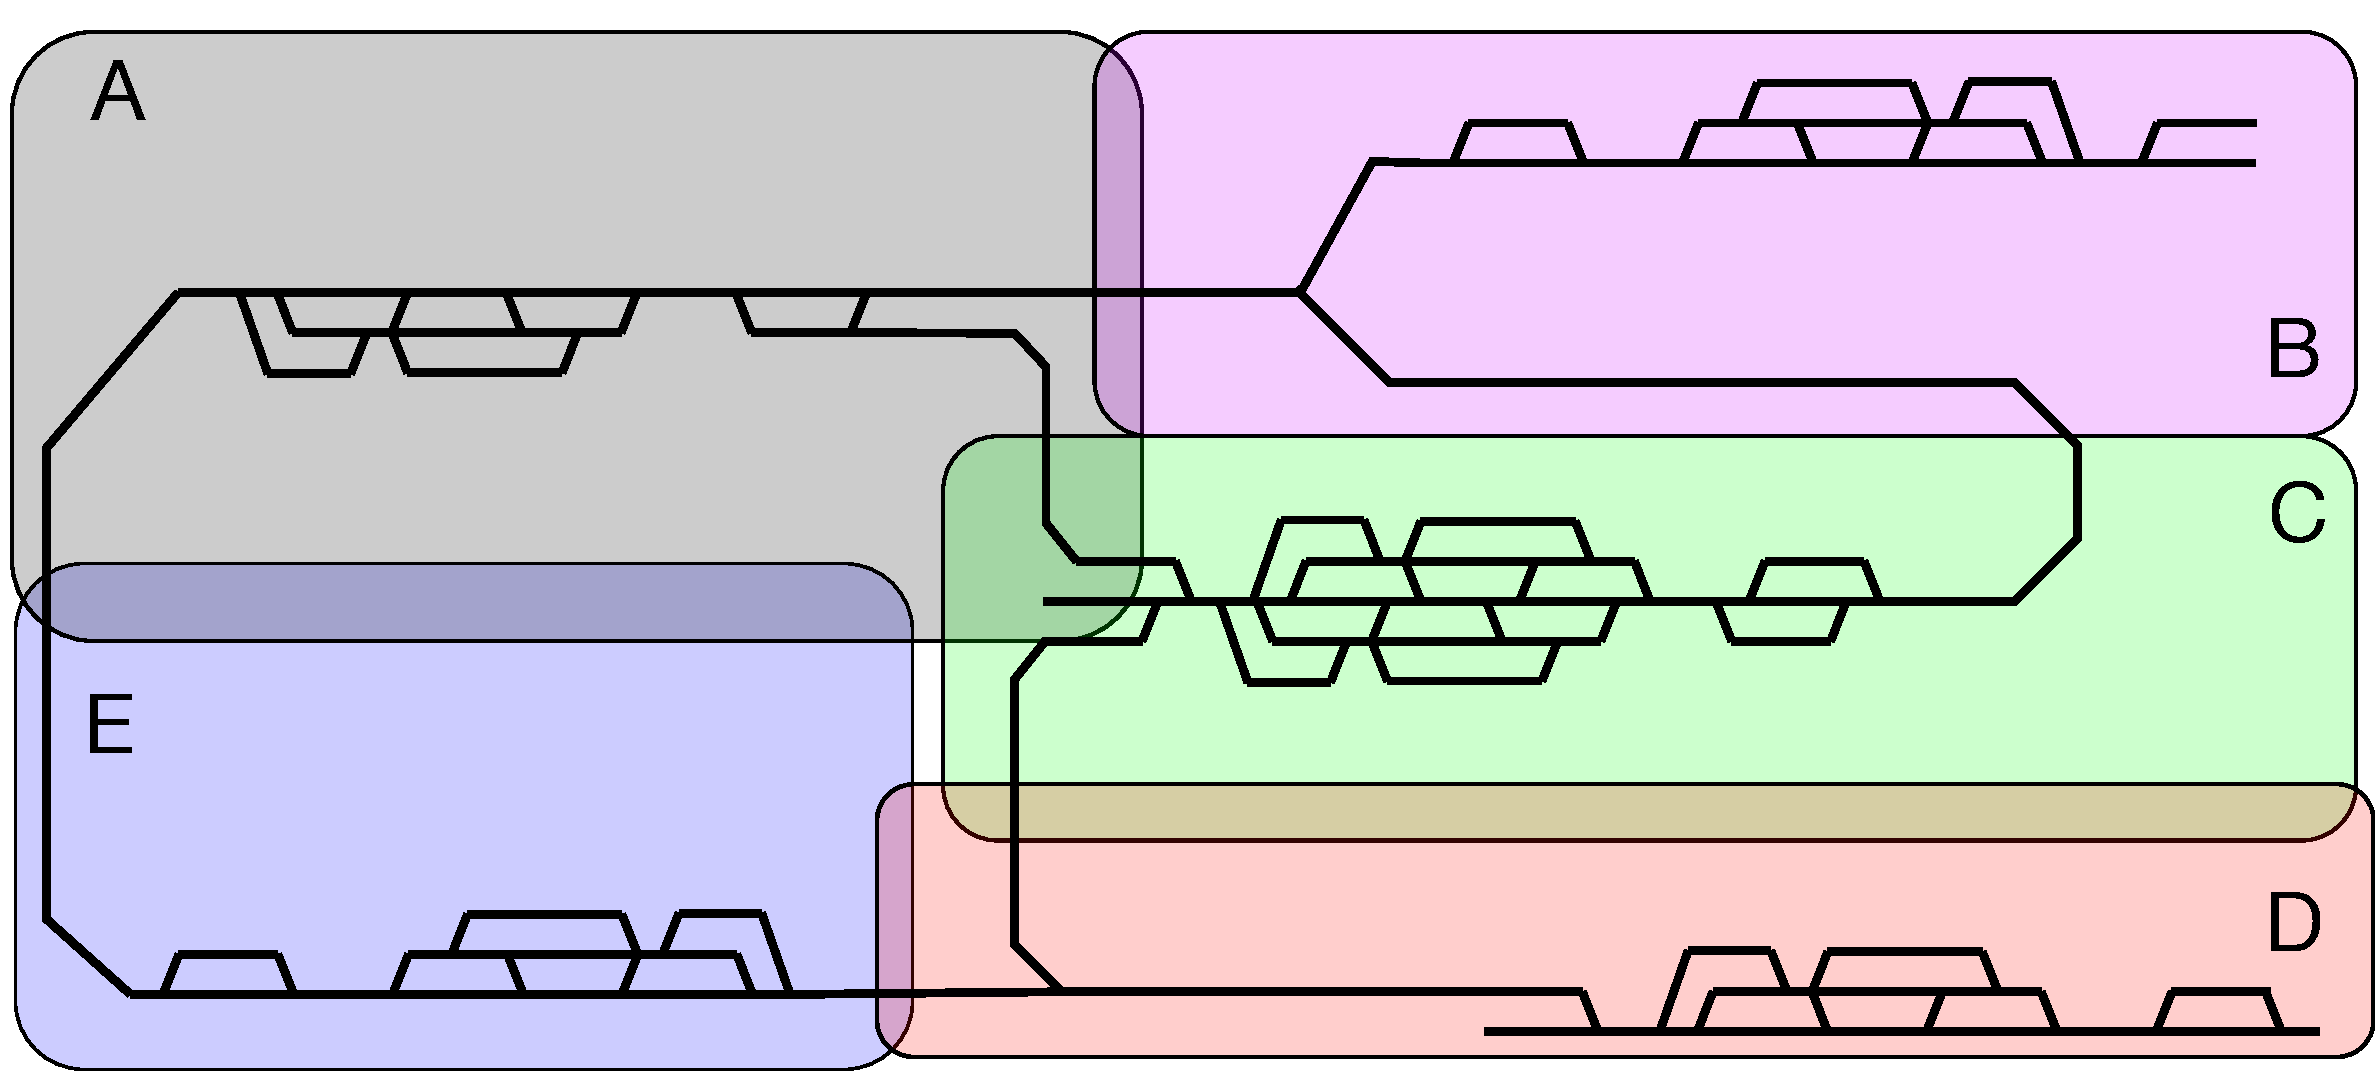
\includegraphics[width=\textwidth]{Figures/disposition_areas.pdf}
	\caption{\textit{Due to the vast complexity of a railway network the re-scheduling task is decomposed into smaller geographical areas (A-E), withiwin which human dispatchers optimize traffic flow. Inter-region coordination is mostly done by informal means of communication such as telephone.} }
	\label{fig:geographical_decomposition}
\end{figure}
%

This situation is depicted in a schematic way in Figure~\ref{fig:introduction_compensation}:
%
\begin{figure}[hbtp]
	\centering
  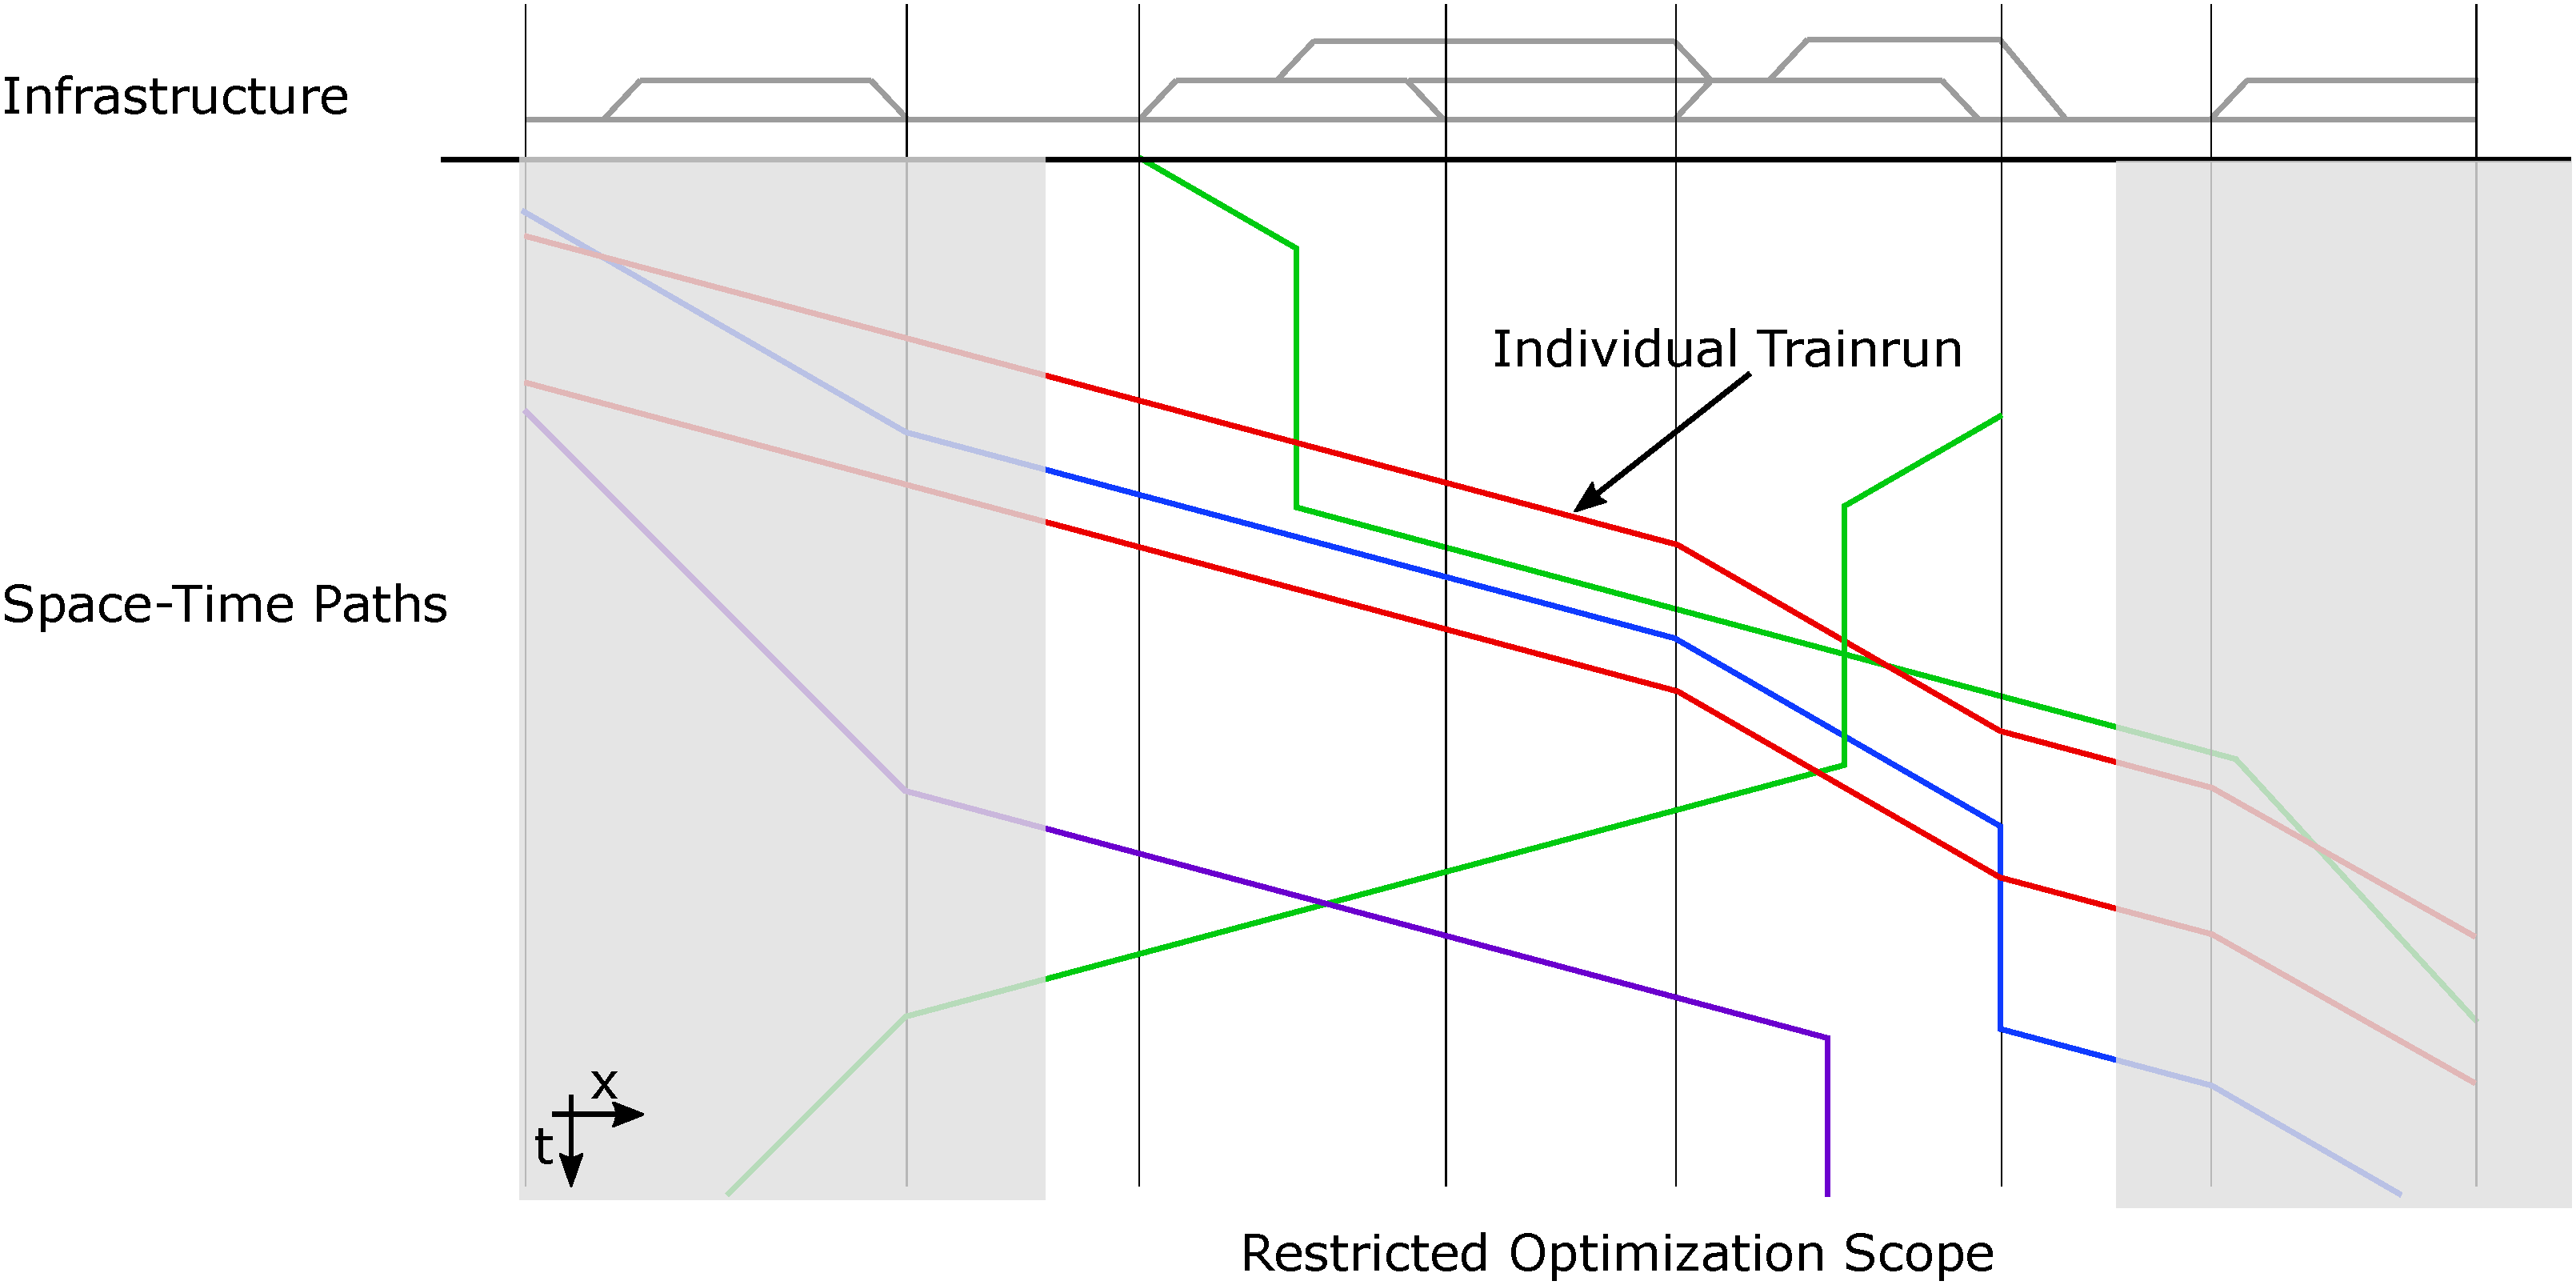
\includegraphics[width=\textwidth]{Figures/rsp_rescheduling_heute.pdf}
	\caption{\textit{Real-time rescheduling has so far been applied to restricted geographic areas only. This means that human intervention or buffer times are necessary outside of the optimization scope to guarantee conflict free traffic in the whole network. The limited geographical scope leads to a cost-function that can only locally be minimized and might have negative effects on the whole network scale.} }
	\label{fig:introduction_compensation}
\end{figure}
%


%
\begin{quote}
    [...], a network separation approach is applied to divide the railway network into zones of manageable size by taking account of the network properties, distinguishing condensation and compensation zones. Condensation zones are usually situated near main stations, where the track topology is complex and many different routes exist. As such an area is expected to have a high traffic density, it is also a capacity bottleneck and trains are required to travel through with maximum allowed speed and thus without time reserves. Collisions are avoided by exploiting the various routing possibilities in the station area. Conversely, a compensation zone connects two or more condensation zones and consists of a simpler topology and less traffic density. Here, time reserves should be introduced to improve timetable stability. The choice of an appropriate speed profile is the most important degree of freedom to exploit in these compensation zones. \cite{caimi2009}
\end{quote}

 There are only a few so-called condensation areas \cite{caimi2009} (in bottleneck areas such as merging/approach areas in front of large stations or tunnels) that are operated through automatic systems. Between these dense areas, trains need to be able to compensate for temporal delays: if trains are reordered or rerouted, these decisions must be feasible in the neighboring areas.

The following Figure~\ref{fig:introduction_operations} shows the re-scheduling control loop adapted from \cite{rcsbrochure,rcswhitepaper}. 
%
\begin{figure}[hbtp]
	\centering
%  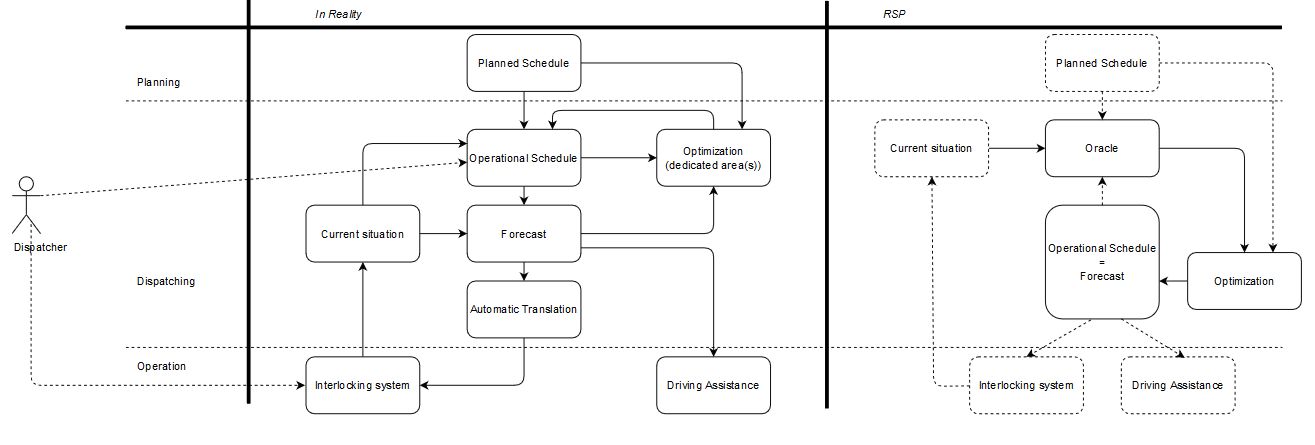
\includegraphics[width=0.9\textheight,angle=90]{introduction_operations.PNG}
  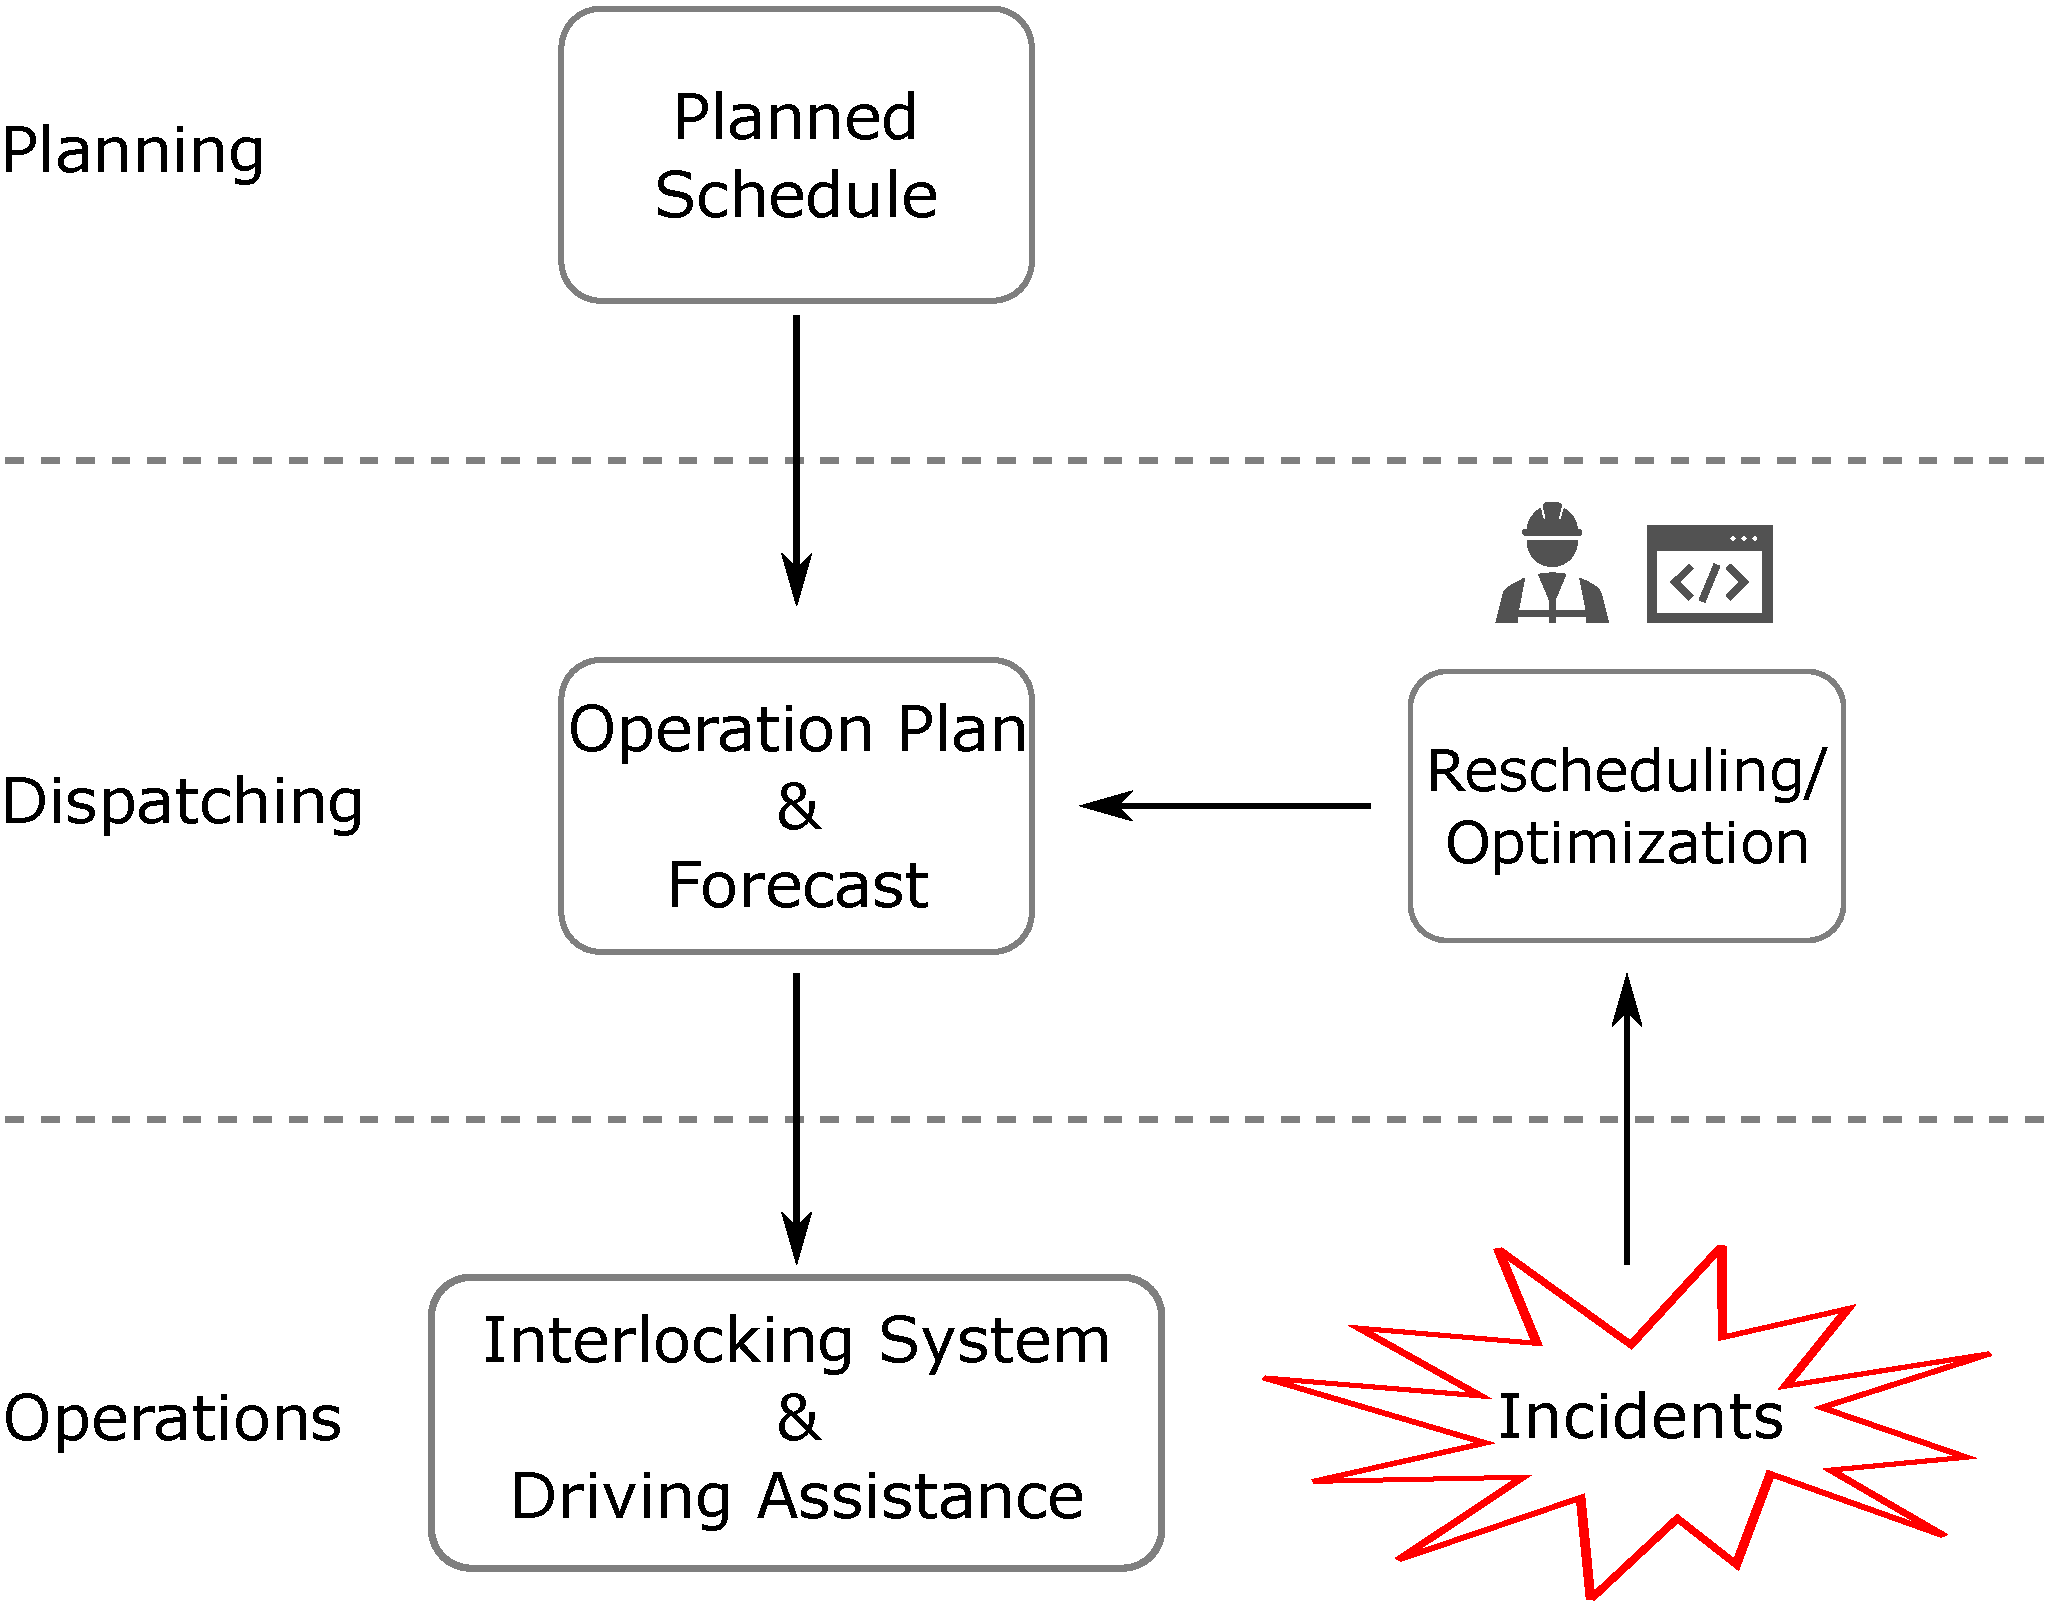
\includegraphics[width=0.8\textwidth]{Figures/rescheduling_schema_heute.pdf}
	\caption{\textit{Simplified schema of the rescheduling process during operations. There are three main areas involved: \emph{planning}, \emph{dispatching} and \emph{operation} (interlocking and driving assistance). Dispatchers have access to the current situation and an automated forecast and make decisions on the level of the operational plan, which are then translated either automatically or by dedicated dispatching team members to the interlocking system; some areas are under the control of an automatic optimization system. As time goes on, new elements from the planned schedule will be introduced to the operational schedule and the planned schedule gives also constraints to re-scheduling: passenger trains must not depart earlier than communicated to customers and the service intention may define further hard or soft constraints such as pecuniar penalties for delay or train dropping. The current situation will be reflected in the operational schedule and the forecast.}}
	\label{fig:introduction_operations}
\end{figure}
%

Our playground implementation is a simplification (see Section~\ref{subsec:playground} below), shown in Figure~\ref{fig:introduction_operations}: we only consider an operational plan and a single delay and try to re-schedule such that we have a conflict-free plan again that stays close to the (published) planned schedule. We hint at a fully automatic re-scheduling loop as follows: information from the current situation needs to be included into the operational plan by passing it to the optimizer; as time moves on, new trains from the planned schedule need to be included into the operational schedule.

In reality, a distinction is made between
\begin{itemize}
    \item operational schedule containing train routes and train ordering
    \item forecast containing passing times within a time horizon
\end{itemize}
%
The forecast outside the optimization areas needs only be conflict-free for the imminent decisions; conflicts in the future are continually resolved by human dispatchers.

As these areas handled by automatic train operation are expected to grow, we think that the locality of decision-making might become a problem since it will be increasingly difficult to define the interfacing conditions that allow to treat the area as an independent optimization problem.
%
Therefore, in our RSP approach, we consider how not to take space-local decisions; also we think of operational schedule and forecast as the same, being conflict-free.


%%%%%%%%%%%%%%%%%%%%%%%%%%%%%%%%%%%%%%%%%%%%%%%%%%%%%%%%%%%%%%%%%%%%%%%%%%
%%%%%%%%%%%%%%%%%%%%%%%%%%%%%%%%%%%%%%%%%%%%%%%%%%%%%%%%%%%%%%%%%%%%%%%%%%
\section{Research Approach}\label{sec:researchapproach}
%%%%%%%%%%%%%%%%%%%%%%%%%%%%%%%%%%%%%%%%%%%%%%%%%%%%%%%%%%%%%%%%%%%%%%%%%%
%%%%%%%%%%%%%%%%%%%%%%%%%%%%%%%%%%%%%%%%%%%%%%%%%%%%%%%%%%%%%%%%%%%%%%%%%%

%%%%%%%%%%%%%%%%%%%%%%%%%%%%%%%%%%%%%%%%%%%%%%%%%%%%%%%%%%%%%%%%%%%%%%%%%%
\subsection{Research Approach: Core idea}\label{subec:coreidea}
%%%%%%%%%%%%%%%%%%%%%%%%%%%%%%%%%%%%%%%%%%%%%%%%%%%%%%%%%%%%%%%%%%%%%%%%%%

Physical railway infrastructure is expensive in building and maintenance \cite{sr40programm}. 
Therefore, the existing infrastructure capacity should be exploited as best as possible.
As the number of trains operating increases and condensation areas increase in number and size, it will become increasingly difficult to compensate for decisions taken within condensation zones or to define restrictions that keep the effects on the neighboring compensation zones as predictable as possible.


The general line of argument will be as follows
\begin{enumerate}
\item it is possible to predict the affected time-space, either from the problem structure or from historic data
\item such a prediction allows for a speed-up of the OR model
\end{enumerate}


To tackle this problem, our approach is to combine Operations Research and Domain-specific Learning to get the best of both worlds: an ``Oracle'' is able to predict the ``impact'' of a delay, with or without a knowledge base learnt by training; we hope the Oracle could predict which trains and which departures are or could be affected by the delay based on past decisions. This piece of information from the Oracle then helps the solver to constrain the search space or at least drive its search more efficiently (driving the branching process).


\begin{mdframed}
{\bf TODO Erik}  Add information about what we mean by automated problem scope reduction: Heuristic, historical, structures, .....

\end{mdframed}

%%%%%%%%%%%%%%%%%%%%%%%%%%%%%%%%%%%%%%%%%%%%%%%%%%%%%%%%%%%%%%%%%%%%%%%%%%
\subsection{Research Approach: a Synthetic Playground}\label{subsec:playground}
%%%%%%%%%%%%%%%%%%%%%%%%%%%%%%%%%%%%%%%%%%%%%%%%%%%%%%%%%%%%%%%%%%%%%%%%%%

We now give a short introduction to our playground implementation (G4) and its limitation with respect to real-world features.
\begin{description}
\item[Synthetic Infrastructure and Simplified Resource Model] We use the FLATland toolbox \cite{aicrowdFLATland} to generate a grid world infrastructure consisting of 2D square cells; the infrastructure defines the possible movements to the 4 neighbor cells mirroring railway infrastructure (switches etc.)
\item[Synthetic Timetable and Train Dynamics]
\begin{itemize}
    \item Every train has one single source and target, no intermediate stops, as provided by the FLATland toolbox \cite{aicrowdFLATland}.
    \item Every train has a constant speed (which may be different from train to train), as provided by the FLATland toolbox \cite{aicrowdFLATland}.
    \item The schedule (departure and passing times at all cells) is generated such that the sum of travel times of all trains is minimized within a chosen upper bound; this the generated timetable might not have a realistic structure.
    \item There are no time reserves in the schedule, trains cannot catch up.
    \item There is no distinction between published timetable and operational schedule, we only have an operational timetable; in reality, trains must not depart earlier than published.
    \item There are no connections or vehicle tours (turnrounds).
\end{itemize}
\item[Synthetic route alternatives] We use shortest paths (in reality, in particular in the case of disturbances affecting a whole area, we might need a different scheme knowing the parts that cannot be taken); path cycles are not allowed.
\item[Simple Disturbance Model] We simulate one train $a$ being stopped for $d$ discrete time steps at some time $t$ and call this a malfunction $M=(t,d, a)$; in reality, the delay might not be known or only probabilities can be assumed. In reality, update information also comes in batches and we would need to consider multiple delays in the same update interval. This setup is shown in Figure~\ref{fig:introduction_no_loop}.
\end{description}
%
\begin{figure}[hbtp]
	\centering
  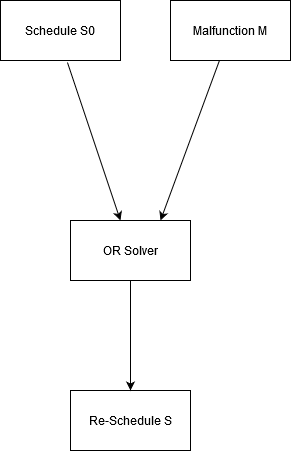
\includegraphics[width=0.4\textwidth]{introduction_no_loop.png}
	\caption{Simple non-iterative re-scheduling with single delay.}
	\label{fig:introduction_no_loop}
\end{figure}

%%%%%%%%%%%%%%%%%%%%%%%%%%%%%%%%%%%%%%%%%%%%%%%%%%%%%%%%%%%%%%%%%%%%%%%%%%
\subsection{Research Approach: Decomposition in Space and Time}\label{subec:scopers}
%%%%%%%%%%%%%%%%%%%%%%%%%%%%%%%%%%%%%%%%%%%%%%%%%%%%%%%%%%%%%%%%%%%%%%%%%%

\begin{mdframed}
{\bf TODO Erik} naming (Oracle -> scoper), figures
\end{mdframed}

We will now detail the general line of argument of Section~\ref{subec:coreidea} by introducing two hypotheses 
\begin{description}
\item [H1] offline scoping: if we have access to an offline solution of the re-scheduling problem given unbounded resources, we can design a scope reduction that allows for a large speed-up (see below, Section~\ref{subec:H1}); by this, we achieve goal \textbf{G2}.
\item [H2] online scoping: it is possible to design a scope reduction, either from the problem structure or from historic data (see below, Section~\ref{subec:H2}); by this, we would over-achieve goal \textbf{G3}.
\end{description}

This approach is shown in Figure~\ref{fig:introduction_time_space}:
%
\begin{figure}[hbtp]
	\centering
  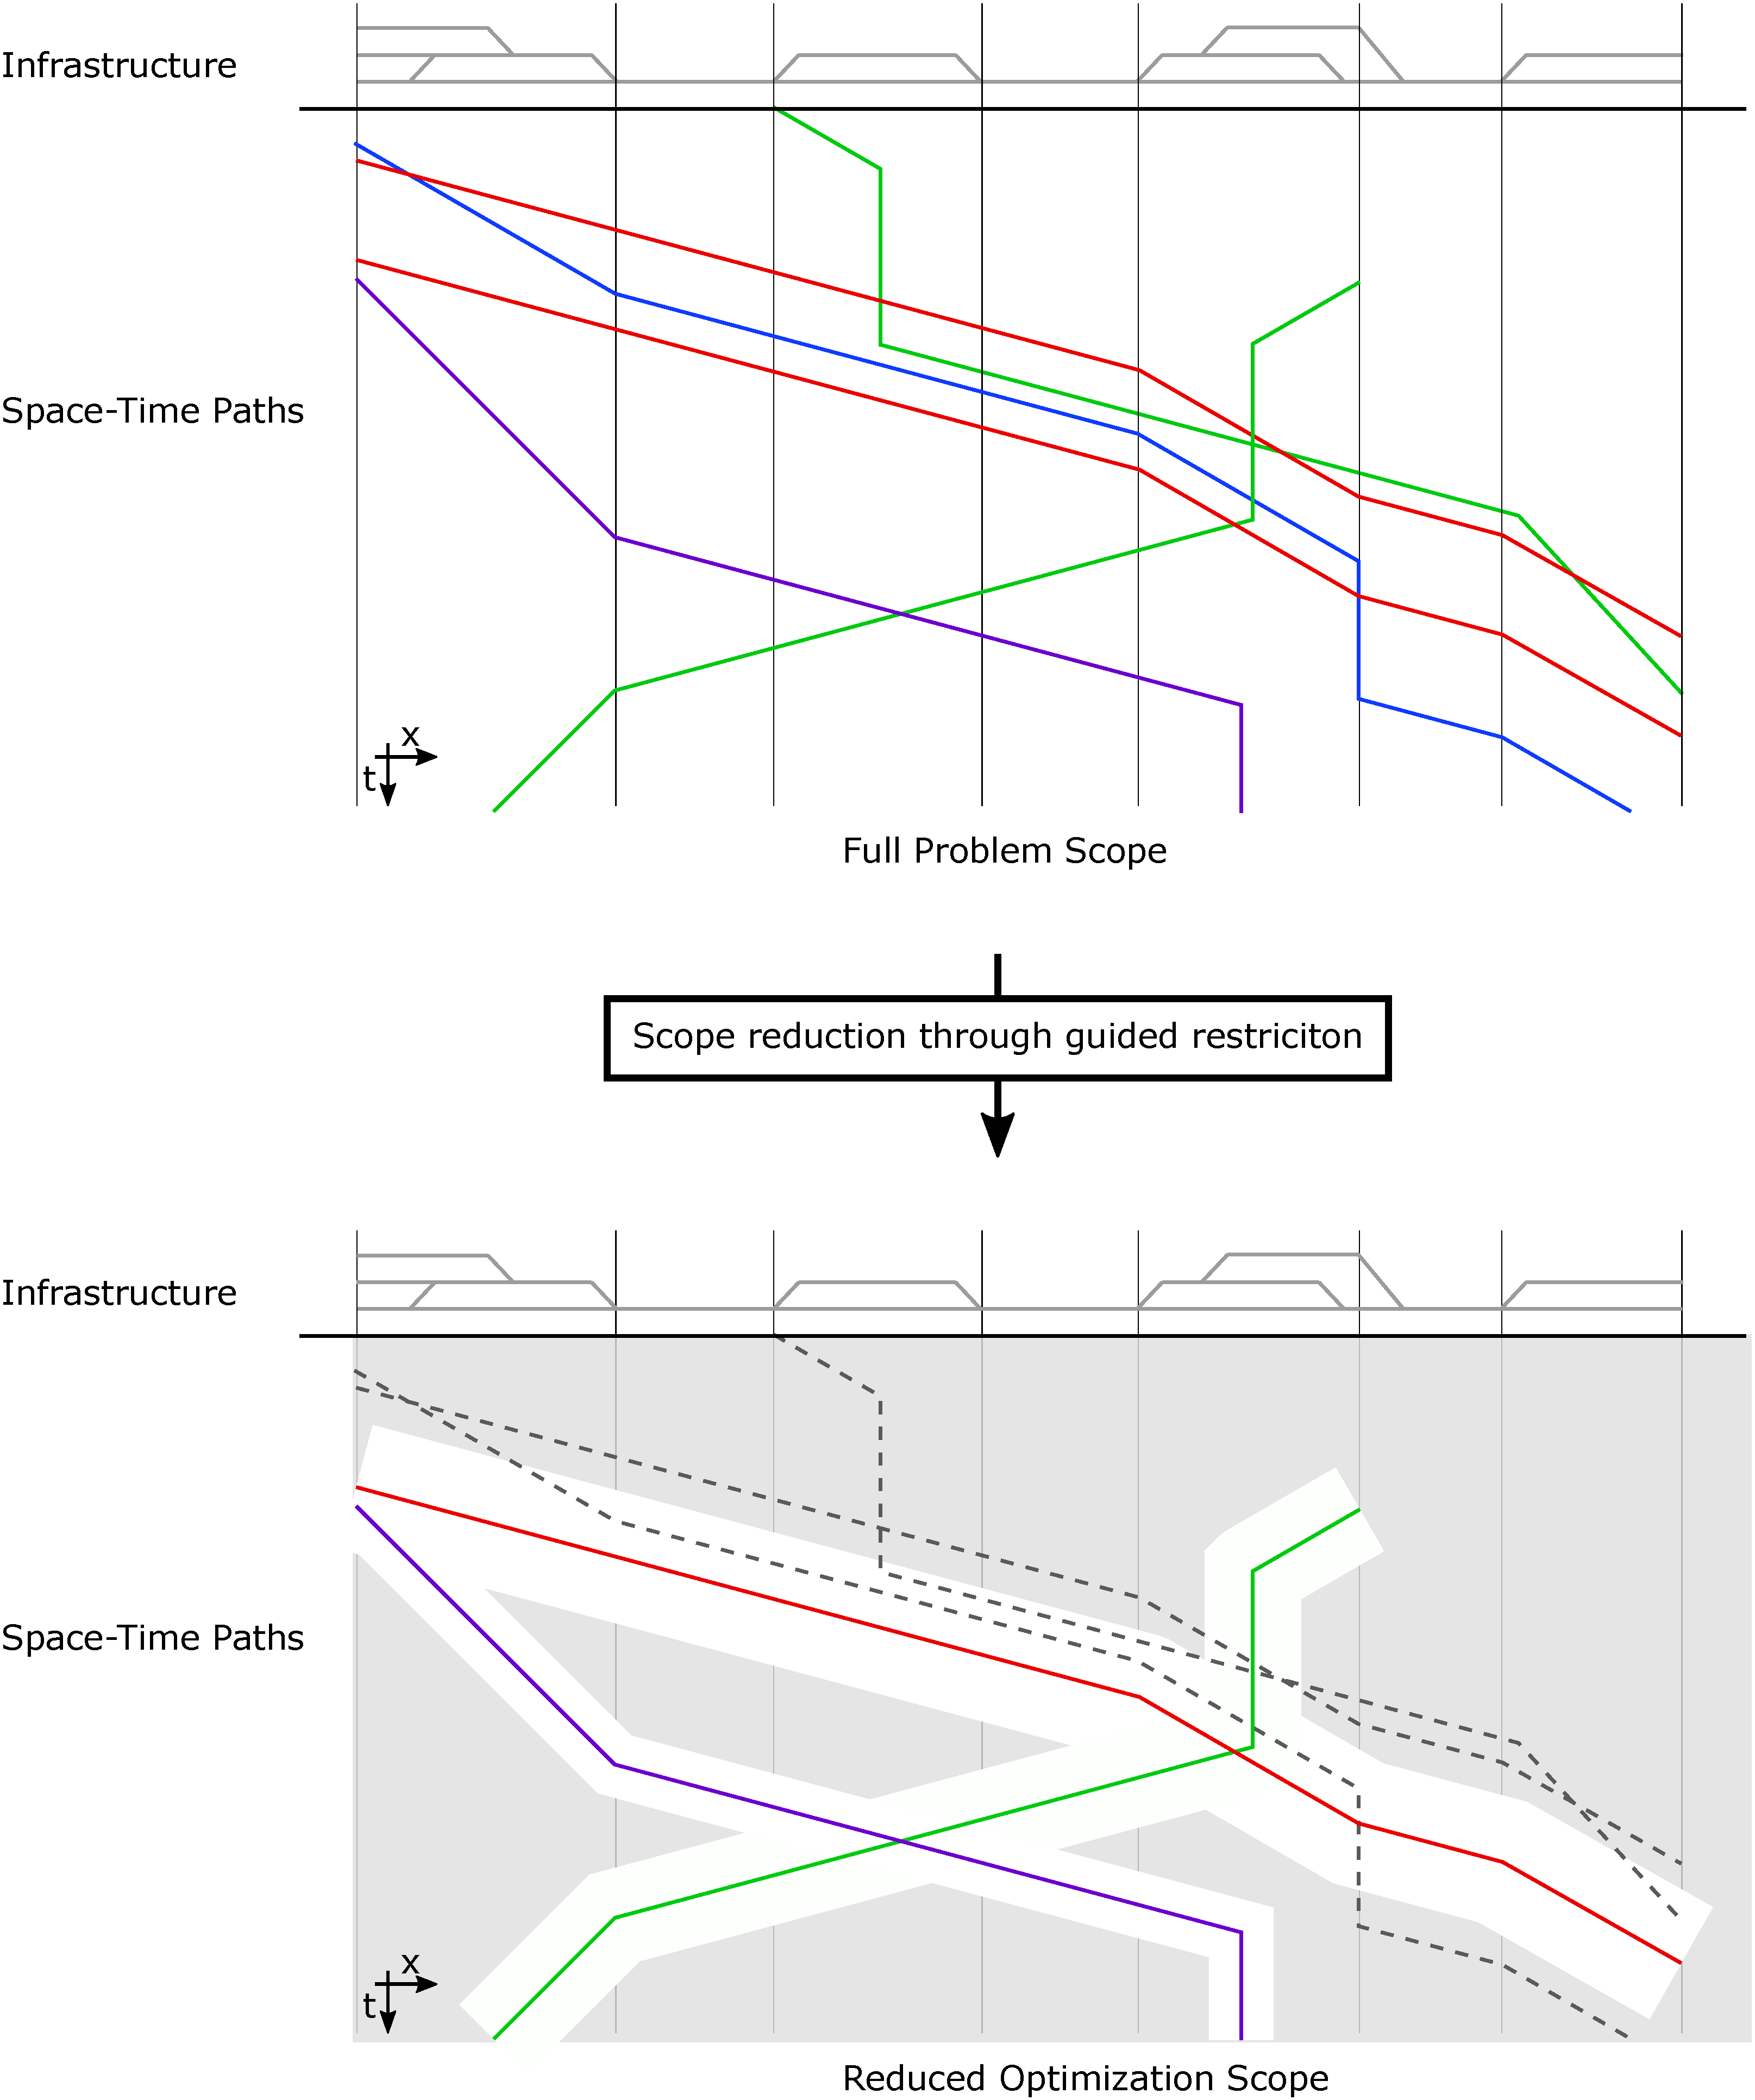
\includegraphics[width=\textwidth]{Figures/rsp_rescheduling_rsp.pdf}
	\caption{The Oracle gives degrees of freedom in time and space.}
	\label{fig:introduction_time_space}
\end{figure}
the Oracle predicts restrictions in time and space, which are passed to the solver.


\begin{mdframed}
{\bf TODO Christian} finalize naming? do we need delta naive?
\end{mdframed}

We will consider the following scopings:
\begin{description}
\item[full after malfunction] this is the full offline solution where we consider the full situation after the malfunction; this excludes paths not reachable any more after the malfunction.
\item[delta perfect] this is the almost perfect scoper which opens up only differences between the initial schedule and the full re-scheduling solution
\begin{itemize}
    \item only paths from either schedule or full after malfunction are allowed;     
    \item if location and time is the same in schedule and full-reschedule, then we stay at them
\end{itemize}
In this case, the solution from full after malfunction is contained in the solution space, so we expect the same (or an equivalent solution modulo costs) to be found.
\item[delta naive] offline scoping, a bit less perfect: for each agent,
\begin{itemize}
    \item if change between schedule and full after malfunction, no restriction after malfunction;    \item if no change between schedule and full after malfunction, we do not open up any freedom for these agents
\end{itemize}
Again, the solution from full after malfunction is contained in the solution space, so we expect the same (or an equivalent solution modulo costs) to be found.
\item[delta online] online scoping: we propagate the delay from one train to the next along paths and times in schedule and open up agents that are predicted affected by the heuristic; we expect the solution quality to deterioriate if there are false negatives.
\item[delta random] this is a sanity check online scoping: if we predict affected trains randomly, we expect solutions to be worse than the ones found by the other scopes or that no solution can be found at all; for example if a train is scheduled to pass through the malfunction train during its malfunction and is not opened, there is no solution even if we enlarge time windows.
\end{description}
These scopers will be introduced formally with pseudo-code below in Section~\ref{subec:scopers}.



\subsubsection{Hypothesis H1: Rationale of Offline Scoping}\label{subec:H1}

Hypothesis 1 is a sanity hypothesis: if we do not have a big speed-up with a perfect oracle, the whole approach must be dismissed. If no speed-up can be found we want to identify the reason and document this to gain further insight and adjust our research aim.

Consider Figure~\ref{fig:introduction_H1}:
%
\begin{figure}[hbtp]
	\centering
  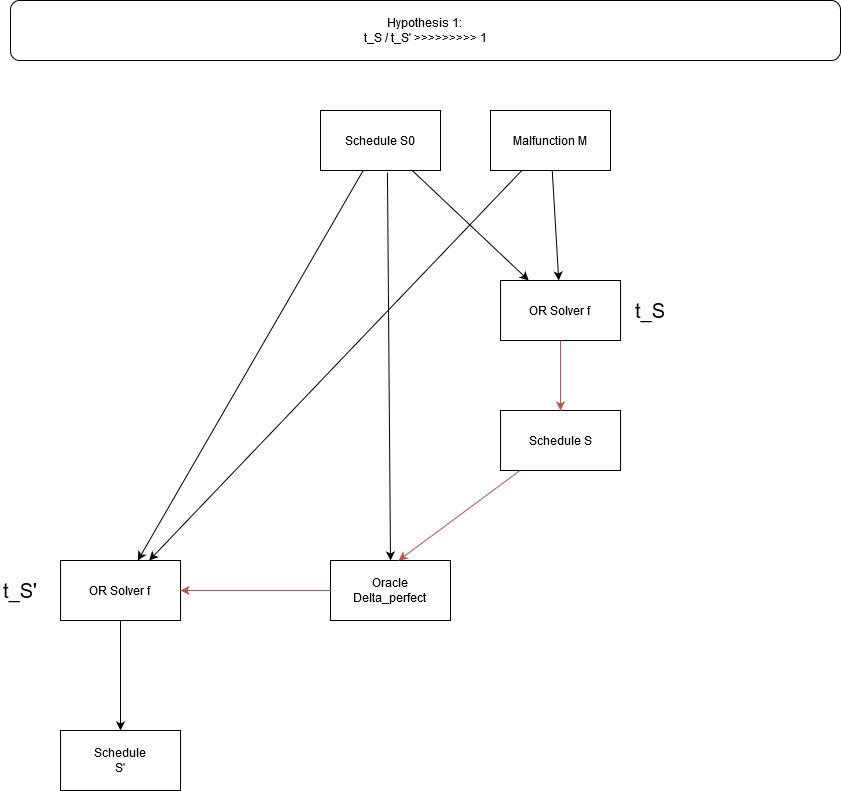
\includegraphics[width=0.9\textwidth]{introduction_H1.png}
	\caption{Rationale of hypothesis H1.}
	\label{fig:introduction_H1}
\end{figure}
%
The initial schedule $S0$ and a malfunction $M$ are passed to an OR solver which is given unbounded time to solve the model to optimality; the resulting re-schedule is $S$.

If we compare the initial schedule $S0$ and the re-schedule $S$, we can take the differences ($Delta\_perfect$):

\begin{itemize}
    \item     every time difference at the same node opens up timing flexibility: the nodes are kept fixed, but time is flexible
    \item every node difference opens up routing flexibility: both nodes and times are kept flexible
\end{itemize}
We will describe this in more detail below in Section~\ref{subsubsec:Delta0}.


Now we want to see whether the OR solver $f$, given the perfect information coming through the red arrows, allows for a speed-up, i.e. whether the time $t\_{S^\prime}$  needed for the solver with the restriction is much smaller than the time $t\_S$ for the full problem without the restriction 

The rationale of this hypothesis is non-general and asymmetric:
%
\begin{itemize}
    \item 
    \emph{non-general}: if we show the speed-up for one particular OR solver, this does not mean that the information can be exploited by every other OR solver for speed-up. However, we conjecture that general setup may be applicable to other OR solvers and models, where the exact content of the Oracle's "hint" passed to the solver might differ. We might strengthen this conjecture by comparing with
\item
    \emph{asymmetric}: If we cannot show the speed-up for one particular solver, this does not exclude that the approach might work with a different OR solver and its particular shape of "perfect information". We might need to consider a different OR solver for our exposition.
\end{itemize}



\subsubsection{Hypothesis H2: Rationale of Online Scoping}\label{subec:H2}
Hypothesis 2 asks whether we can build an oracle that provides a considerable speed-up without access to perfect information, only from the current situation.

Consider Figure~\ref{fig:introduction_H2}:
%
\begin{figure}[hbtp]
	\centering
  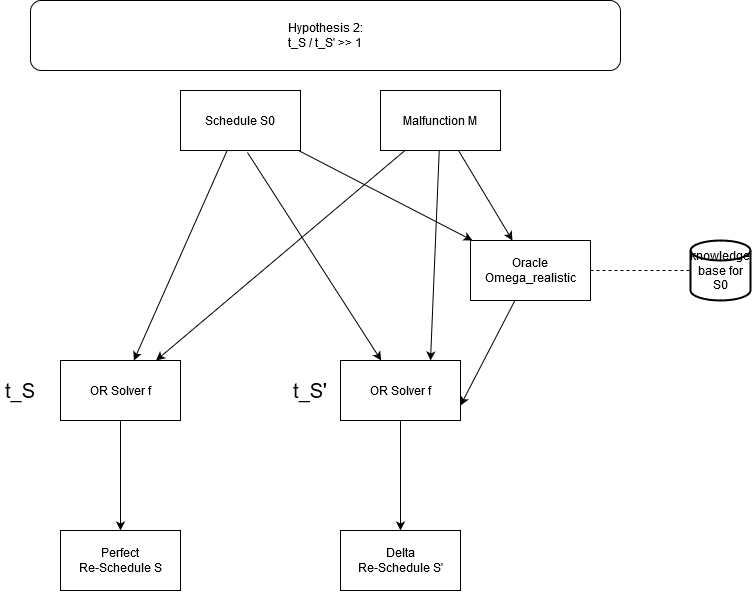
\includegraphics[width=0.9\textwidth]{introduction_H2.png}
	\caption{Rationale of hypothesis H2.}
	\label{fig:introduction_H2}
\end{figure}
%
Our Oracle $Omega\_realistic$ now has only access to the current information and possibly its knowledge base, not to the perfect re-schedule for the current situation. Can it provide hints to the OR solver that allows for a speed-up $t\_S / t\_S' >> 1$?

We will not build such an $Omega\_realistic$, but report on some first ideas which illustrate the limitation of a geographic decomposition in our synthetic setting \ref{sec:CaseStudies}. We hope this motivates researchers to invest in this task.



%%%%%%%%%%%%%%%%%%%%%%%%%%%%%%%%%%%%%%%%%%%%%%%%%%%%%%%%%%%%%%%%%%%%%%%%%%
%%%%%%%%%%%%%%%%%%%%%%%%%%%%%%%%%%%%%%%%%%%%%%%%%%%%%%%%%%%%%%%%%%%%%%%%%%
\section{The Pipeline for H1 and H2}
%%%%%%%%%%%%%%%%%%%%%%%%%%%%%%%%%%%%%%%%%%%%%%%%%%%%%%%%%%%%%%%%%%%%%%%%%%
%%%%%%%%%%%%%%%%%%%%%%%%%%%%%%%%%%%%%%%%%%%%%%%%%%%%%%%%%%%%%%%%%%%%%%%%%%

In this section, we will formalize the ideas of our research approach as outlined in Section~\ref{sec:researchapproach}.


%%%%%%%%%%%%%%%%%%%%%%%%%%%%%%%%%%%%%%%%%%%%%%%%%%%%%%%%%%%%%%%%%%%%%%%%%%
\subsection{Overview}\label{subsubsec:H1overview}
%%%%%%%%%%%%%%%%%%%%%%%%%%%%%%%%%%%%%%%%%%%%%%%%%%%%%%%%%%%%%%%%%%%%%%%%%%
We now give a more detailed view of the pipeline for hypothesis H1 with respect to Section~\ref{subec:H1}. We refer to Figure~\ref{fig:H1_overview}:
%
\begin{mdframed}
{\bf TODO Christian} update diagram
\end{mdframed}
\begin{figure}[hbtp]
	\centering
  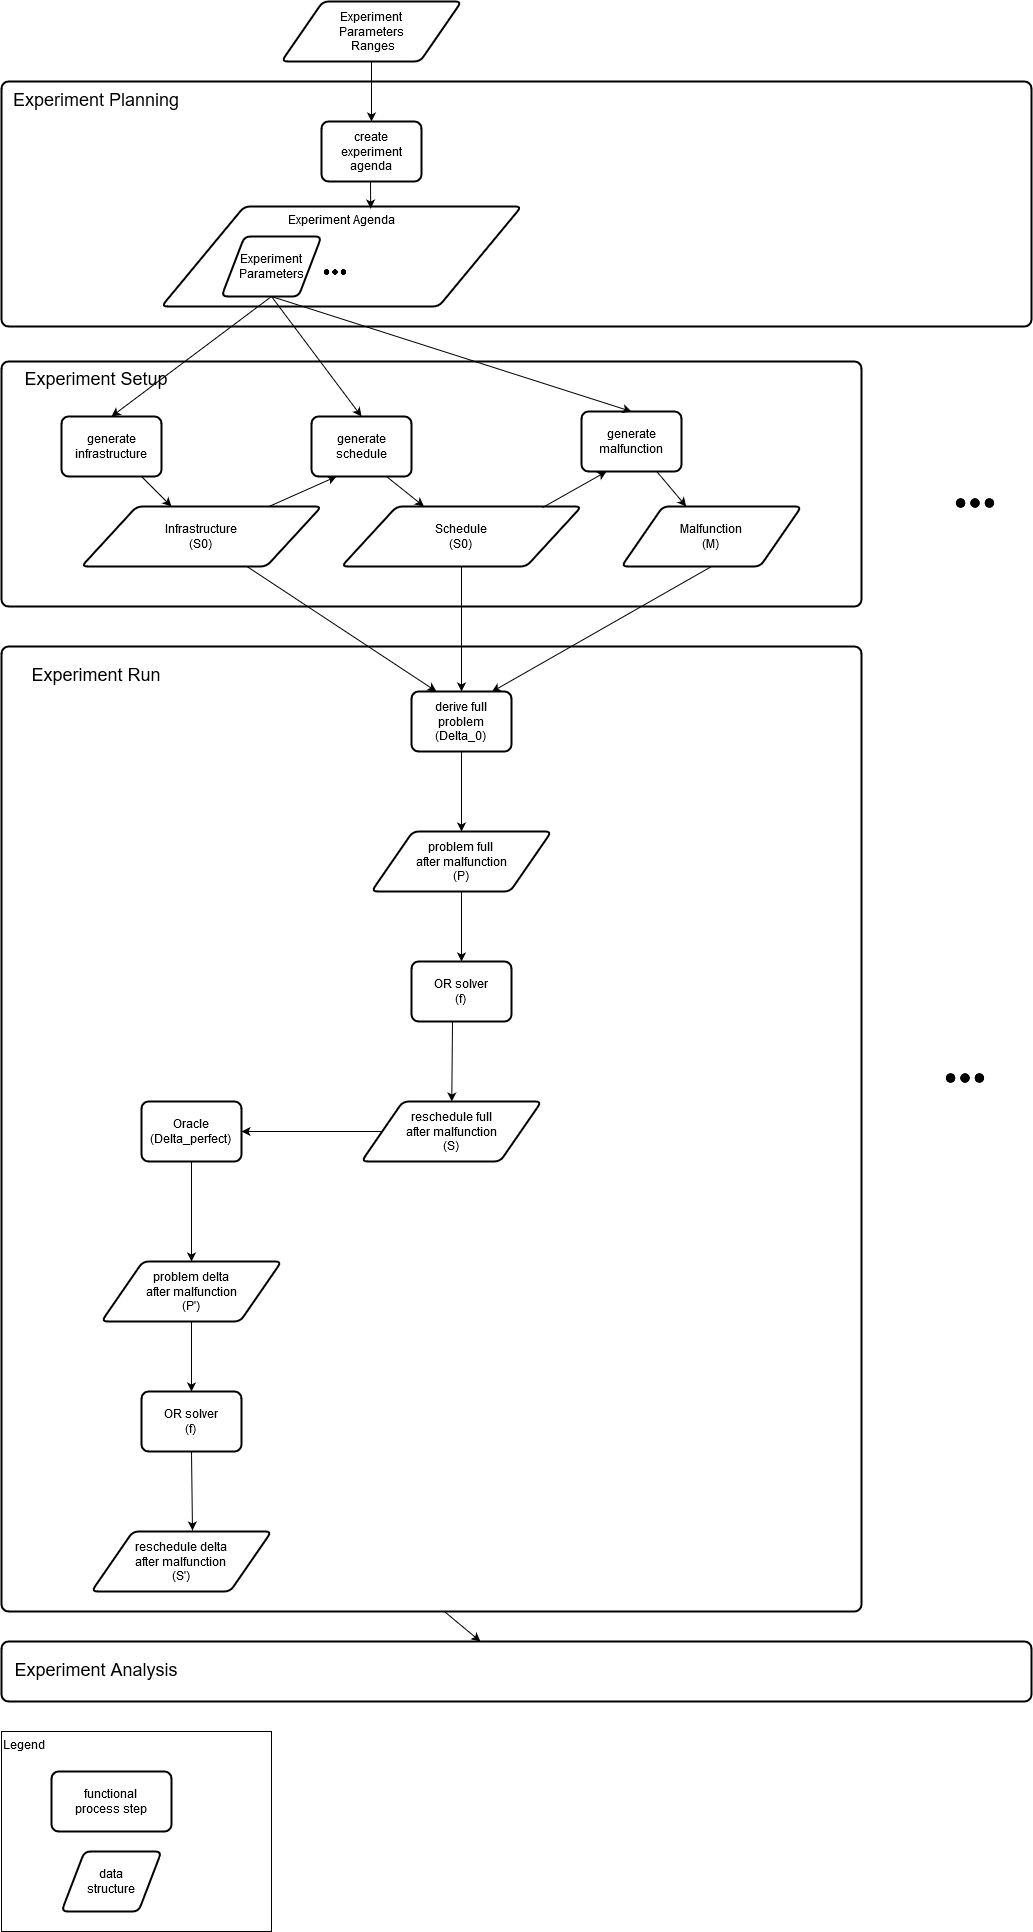
\includegraphics[width=0.8\textwidth]{H1_overview.png}
	\caption{Pipeline for hypothesis H1 as functional diagram with intermediate data structures at two levels. The top level consists of four stages.}
	\label{fig:H1_overview}
\end{figure}
%
the pipeline decomposes into five top-level stages:
\begin{description}
\item[Infrastructure Generation] This generates railway topologies and places agent start and targets in the infrastructure. We will cover this stage in detail in Section~\ref{subsubsec:infrastructuregeneration}
\item[Schedule Generation] This generates the exact conflict-free paths and times through the infrastructure for all agents. We will cover this stage in detail in Sections~\ref{subsubsec:schedulegeneration}. 
\item[Malfunction Generation] Which train is delayed when during its run and for how long?
\item[Experiment Run] Here, the different scopers are run. We will cover these data structures and functional process steps in Sections~\ref{subsubsec:scheduleproblemdescription} and \ref{subec:scopers}.
\item[Experiment Analysis] This stage produces the plots that help to verify hypothesis H1. We will give more details in Sections~\ref{sec:Results} and \ref{sec:CaseStudies}.
\end{description}
Since the schedule generation step takes too long to repeat for every experiment, we will use the same infrastructure and schedule for many malfunctions. In fact, we can pre-generate infrastructures and schedules and then work on variations of the re-scheduling part of the pipeline more efficiently.



%%%%%%%%%%%%%%%%%%%%%%%%%%%%%%%%%%%%%%%%%%%%%%%%%%%%%%%%%%%%%%%%%%%%%%%%%%
\subsection{Infrastructure Generation}\label{subsubsec:infrastructuregeneration}
%%%%%%%%%%%%%%%%%%%%%%%%%%%%%%%%%%%%%%%%%%%%%%%%%%%%%%%%%%%%%%%%%%%%%%%%%%

We now describe our railway infrastructure and how it is generated, mimicking a natural setup. 

The infrastructure consists of a grid of cells. Each cell consists of a distinct tile type which defines the movement possibilities of the agent through the cell. There are 8 basic tile types, which describe a rail network. As a general fact in railway network when on navigation choice must be taken at maximum two options are available. 
%
Figure~\ref{fig:H1_railway_elements} (top) gives an overview of the eight basic types. These can be rotated in steps of $45^\circ$ and mirrored along the North--South of East--West axis. The bottom row shows the corresponding translation into a graph structure: squares represent cells, black dots represent an entry to pin to the depicted cell and a grey dot represents the pin in the opposite direction into the neighboring cell.
%
\begin{figure}[hbtp]
	\centering
  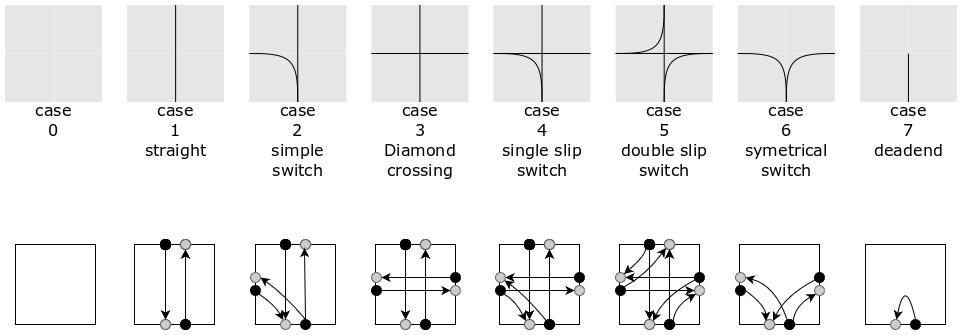
\includegraphics[width=0.8\textwidth]{H1_railway_elements.png}
	\caption{Eight basic cell types of a FLATland grid (top) and their translation into a directed graph (bottom).}
	\label{fig:H1_railway_elements}
\end{figure}
%
Formally, the \emph{railway infrastructure} is a tuple  $(\mathcal{C}, \mathcal{V}, \mathpzc{c}, \mathcal{E})$, where
\begin{itemize}
    \item $\mathcal{C}$ is a set of cells,
    \item $\mathcal{V}$ is the set of pins by which the cell can be entered (they are positioned to the north, east, south or east of the cell),
    \item $\mathpzc{c}: \mathcal{V} \to \mathcal{C}$ which associates to each ``pin'' the cell it enters (there are at most $4$ pins for every cell),
    \item $\mathcal{E} \subseteq \mathcal{V} \times \mathcal{V}$, the possible directed transitions in the grid;
\end{itemize}
furthermore, we require $(\mathcal{V},\mathcal{E})$ to be an acyclic graph.



\begin{mdframed}
{\bf TODO Erik} describe infrastructure generation: placement of stations and lines (FLATland)
\end{mdframed}


            
%%%%%%%%%%%%%%%%%%%%%%%%%%%%%%%%%%%%%%%%%%%%%%%%%%%%%%%%%%%%%%%%%%%%%%%%%%
\subsection{General Train Scheduling Problem}\label{subsubsec:scheduleproblemdescription}
%%%%%%%%%%%%%%%%%%%%%%%%%%%%%%%%%%%%%%%%%%%%%%%%%%%%%%%%%%%%%%%%%%%%%%%%%%



We will introduce the abstract model from \cite{DBLP:journals/corr/abs-2003-08598}, which we will use both for schedule generation and for re-scheduling; we could use any schedule as input, but we use the same solver model for practical reasons; the difference between these two applications is only in the optimization objective used as detailled in Sections~\ref{subsubsec:schedulegeneration} and \ref{eq:objectiveresched}, respectively.
Furthermore, the model introduced in this section is more general than we actually need for our pipeline for H1; this will allow us to review the synthetic assumptions of Section~\ref{subsec:playground} in a more formal setting.



According to \cite{DBLP:journals/corr/abs-2003-08598},  the \emph{(general) train scheduling problem} is formalized as a tuple $(N, \mathcal{A}, C, F)$ having the following components
\begin{itemize}
    \item $N$ stands for the railway network $(V, E, R, m, a, b)$, where
        \begin{itemize}
            \item $(V, E)$ is a directed graph,
            \item $R$ is a set of resources,
            \item $m:E\to\mathbb{N}$ assigns the minimum travel time of an edge,
            \item $a: \mathbb{R}\to 2^E$ associates resources with edges in the railway network, and
            \item $b:R\to \mathbb{N}$ gives the time a resource is blocked after it was accessed by a train line.
        \end{itemize}
    \item $\mathcal{A}$ is a set of train lines to be scheduled on network $N$. Each train in $\mathcal{A}$ is represented as a tuple $(S, L, e, l, w)$, where
        \begin{itemize}
            \item $(S, L)$ is an acyclic subgraph of $(V, E)$,
            \item $e:S \to \mathbb{N}$ gives the earliest time a train may arrive at a node,
            \item $l:S\to \mathbb{N} \cup \left\{\infty\right\}$ gives the latest time a train may arrive at a node, and
            \item $w:L\to \mathbb{N}$ is the time a train has to wait on an edge. 
        \end{itemize}
        Note that all functions are total unless specified otherwise.
        \item $C$ contains connections requiring that a certain train line $a^\prime$ must not arrive at node $n^\prime$ before another train line $a $ has arrived at node $n$ for at least $\alpha$ and at most $\omega$ discrete time steps. More precisely, each connection in $C$ is of form $(t,(v, v^\prime), t^\prime,(u, u^\prime), \alpha, \omega, n, n^\prime)$ such that $a= (S, L, e, l, w)\in \mathcal{A}$ and $a^\prime= (S^\prime, L^\prime, e^\prime, l^\prime, w^\prime)\in \mathcal{A}$, $a\not=a^\prime$,$(v, v^\prime)\in L$,$(u, u^\prime)\in L^\prime$,$\left\{\alpha,\omega\right\} \subseteq \mathbb{Z} \cup \left\{\infty,-\infty\right\}$, and either $n=v$ or $n=v^\prime$, as well as, either $n^\prime=u$ or $n^\prime=u^\prime$.
    \item Finally, $F$ contains collision-free resource points for each connection in $C$. We represent it as a family $(F_c)_{c\in C}$. Connections removing collision detection are used to model splitting (or merging) of trains, as well as reusing the whole physical train between two train lines. More importantly, this allows us to alleviate the restriction that subgraphs for train lines are acyclic, as we can use two train lines forming a cycle that are connected via such connections. Refer to \cite{DBLP:journals/corr/abs-2003-08598} for more details.
\end{itemize}
In this setting, edges can be interpreted as time slices of a train run referring to a certain a speed profile since the resources to be reserved ahead may depend on the speed profile; however, the model has no reference to the underlying geography (coordinates etc.); also, resources have no location -- they can be interpreted as track sections that need to be reserved, but they may also be gates or sideway tracks that need to be reserved while travelling the edge. Notice that different trains may have the same edges in their route DAG, which means that they can drive with the same speed profile at the same place.





We now define solutions:
As above, the \emph{solution to a train scheduling problem} $(N, \mathcal{A}, C, F)$ is a pair $(P,A)$ consisting of 
\begin{enumerate}
    \item a function $P$ assigning to each train line the path it takes through the network, and
    \item an assignment $A$ of arrival times to each train line at each node on their path.
\end{enumerate}
A path is a sequence of nodes, pair-wise connected by edges. We write $v\in p$ and $(v, v^\prime)\in p$ to denote that node $v$ or edge $(v, v^\prime)$ are contained in path $p=(v_1, . . . , v_n)$, that is, whenever $v=v_i$ for some $1\leq i \leq n$, or this and additionally $v^\prime=v_{i+1}$, respectively.
%
A path $P(a) = (v_1, . . . , v_n)$ for $a= (S, L, e, l, w)\in \mathcal{A}$ has to satisfy
\begin{equation}
v_i \in S \textrm{ for }1\leq i \leq n \label{eq:ASP_1},
\end{equation}
\begin{equation}
(v_j, v_{j+1})\in L \textrm{ for } 1\leq j \leq n-1 \label{eq:ASP_2} 
\end{equation}
\begin{equation}
in(v_1) = 0 \textrm{ and } out(v_n) = 0,\label{eq:ASP_3} 
\end{equation}
where $in$ and $out$ give the in- and out-degree of a node in graph $(S, L)$, respectively.
We will write $\tau(a,P)=v_n$ for the target node used by agent $a$ in the schedule $(P,A)$, and, similarly $\sigma(a,P)=v_1$ for the source node of agent $a$ in the schedule $(P,A)$.
Intuitively, conditions (\ref{eq:ASP_1}) and (\ref{eq:ASP_2}) enforce paths to be connected and feasible for the train line in question and Condition (\ref{eq:ASP_3}) ensures that each path is between a possible start and end node.  
An assignment $A$ is a partial function $\mathcal{A}\times V\to \mathbf{N}$, where $A(a, v)$ is undefined whenever$v\not\in P(a)$. In addition, given path function $P$, an assignment $A$ has to satisfy the conditions in (\ref{eq:ASP_4}) to (\ref{eq:ASP_8}):
\begin{equation}
A(a, v_i)\geq e(v_i)\label{eq:ASP_4}
\end{equation}
\begin{equation}
A(a, v_i)\leq l(v_i)\label{eq:ASP_5}
\end{equation}
\begin{equation}
A(a, v_j) +m((v_j, v_{j+1})) +w((v_j, v_{j+1}))\leq A(a, v_{j+1})\label{eq:ASP_6}
\end{equation}
for all $a= (S, L, e, l, w)\in\mathcal{A}$ and $P(a) = (v_1, . . . , v_n)$ such that $1\leq i\leq n$,$1\leq j\leq n-1$,
either
\begin{equation}
A(a, v^\prime) +b(r) \leq A(a^\prime, u) \textrm{ or }A(a^\prime, u^\prime) +b(r)\leq A(a, v) \label{eq:ASP_7}
\end{equation}
for all $r\in R$, ${a, a^\prime} \subseteq \mathcal{A}$, $a\not=a'$,$(v, v^\prime)\in P(a)$,$(u, u^\prime)\in P(a^\prime)$ with $\left\{(v, v^\prime),(u, u^\prime)\right\} \subseteq a(r)$ whenever for all $(a,(x, x^\prime), a^\prime,(y, y^\prime), \alpha, \omega, n, n^\prime)\in C$ such that $(x, x^\prime)\in P(a)$,$(y, y^\prime)\in P(a^\prime)$, we have $(a,(v, v^\prime), a^\prime,(u, u^\prime), r)\not\in F_c$, and finally
\begin{equation}
\alpha\leq A(t^\prime, n^\prime)-A(t, n)\leq \omega\label{eq:ASP_8}
\end{equation}
for all $(a,(v, v^\prime), a^\prime,(u, u^\prime), \alpha, \omega, n, n^\prime)\in C$ if $(v, v^\prime)\in P(a)$ and $(u, u^\prime)\in P(a^\prime)$.
%
Intuitively, conditions (\ref{eq:ASP_4}), (\ref{eq:ASP_5}) and (\ref{eq:ASP_6}) ensure that a train line arrives at nodes neither too early nor too late and that waiting and traveling times are accounted for. Furthermore, Condition (\ref{eq:ASP_7}) resolves conflicts between two train lines that travel edges sharing a resource, so that one train line can only enter after another has left for a specified time span. This condition does not have to hold if the two trains use a connection that defines a collision-free resource point for the given edges and resource. Finally, Condition (\ref{eq:ASP_8}) ensures that train line $a$ connects to $a^\prime$at node $n$ and $n^\prime$, respectively, within a time interval from $\alpha$ to $\omega$. Note that this is only required if both train lines use the specific edges specified in the connections. Furthermore, note that it is feasible that $n$ and $n^\prime$ are visited but no connection is required since one or both train lines took alternative routes.





%%%%%%%%%%%%%%%%%%%%%%%%%%%%%%%%%%%%%%%%%%%%%%%%%%%%%%%%%%%%%%%%%%%%%%%%%%
\subsection{Schedule Generation}\label{subsubsec:schedulegeneration}
%%%%%%%%%%%%%%%%%%%%%%%%%%%%%%%%%%%%%%%%%%%%%%%%%%%%%%%%%%%%%%%%%%%%%%%%%%



A \emph{railway service intention} defines the commercial contract between railway infrastructure manager (IM) and railway undertaking companies (RU). In our simplified setting, we take it as a set $\mathcal{A}$ of trains or agents; each train $a$ has a source $\sigma(a)\in\mathcal{V}$ and a some target in $\tau(a)\subseteq\mathcal{V}$ and a speed $v(a) \in [0,1]$; furthermore, a release time $r$, which specifies how long a cell remains blocked after a train has left it and which we assume the same for all resources in our setting. This is exactly the output of infrastructure generation as described in Section~\ref{subsubsec:infrastructuregeneration}; correctly, we should have introduced an additional layer into our hierarchical approach, splitting our infrastructure generation into infrastructure and service intention; for purely practical reasons only did we refrain from doing this (FLATland does not store the station areas in the final layout, they are only temporary data structures during grid generation, and we would have had to extend FLATland for this purpose).


We now show how a general train scheduling problem can be derived from such a railway service intention. Let $(\mathcal{A},\sigma,\tau,v,r)$ be a service intention in a railway infrastructure $(\mathcal{C}, \mathcal{V}, \mathpzc{c}, \mathcal{E})$.
Then, $(N,\tilde{\mathcal{A}},C,F)$ with
\begin{itemize}
    \item $\tilde{\mathcal{A}}$ consists of a tuple $(S,L,e,l,w)$ for each $a \in \mathcal{A}$ where 
        \begin{itemize}
            \item $S=\left\{ v: v \in P_a\right\}$
            \item $L=\left\{ (v_1,v_2): (v_1,v_2) \in P_a\right\}$
            \item $e(v)=\min_{p: \sigma(a)\textrm{--}v\textrm{ path}} \left|p\right| \cdot {v(a)}^{-1}$ 
            \item $l(v)=\max_{p: v\textrm{--}\tau(a)\textrm{ path}} U-\left|p\right| \cdot {v(a)}^{-1}$
            \item $w(e)={v(a)}^{-1}$\mbox{  }\footnote{This does not respect the intended semantics of the general model. Therefore, it would be better to use $S=\left\{ (v,a): v \in P_a\right\}$, $L=\left\{ ((v_1,a),(v_2,a)): (v_1,v_2) \in P_a\right\}$, $w(e)=0$ and $m(((v_1,a),(v_2,a)))={v(a)}^{-1}$.}.
        \end{itemize}
        for a set $P_a$ of $\sigma(a)$--$\tau(a)$ paths in $\mathcal{E}$.
        \item $N=(V,E,R,m,a,b)$ where
        \begin{itemize}
            \item $V=\bigcup_{a \in \mathcal{A}} V_a$
            \item $E=\bigcup_{a \in \mathcal{A}} E_a$
            \item $R=\mathcal{C}$
            \item $m((v_1,v_2,a))=0$
            \item $a(c) = \left\{ e=(v_1,v_2,a): \mathpzc{c}(v_1)=c \right\}$
            \item $b(c)=r$
        \end{itemize}
    \item $C=\emptyset$
    \item $F=\emptyset$
\end{itemize}
is a train scheduling problem. Some remarks on this transformation:
\begin{itemize}
    \item We only have one resource per edge, i.e. we only reserve the train's own track, per cell.
    \item The earliest and latest windows are designed such that they represent the earliest possible time the train can reach the vertex, respectively, the latest possible time the train must pass in order to be able to reach the target within the time limit. 
\end{itemize}

The time windows given by $e$ and $l$ can be computed by Algorithm~\ref{algo:propagate_earliest} and \ref{algo:propagate_latest}, respectively. They propagate the minimum running forward from an initial set of earliest and backwards from an initial set of latest constraints. An illustration can be found in Figures~\ref{fig:propagate_earliest} and \ref{fig:propagate_latest}, respectively.
The time windows are thus given by
$$e\leftarrow propagate\_earliest(\Set*{e(\sigma(a))=0}, (S,L), \Set*{\sigma(a)}, {v(a)}^{-1})$$ and $$l\leftarrow propagate\_latest(\Set*{e(\tau)=U: \tau \in S, out(\tau)=0}, (S,L), \Set*{\tau \in S: out(\tau)=0},{v(a)}^{-1}).$$ 
Finally, we can remove nodes $v$ with empty time window $e(v)>l(v)$.





\begin{algorithm}
	\caption{$propagate\_earliest$} \label{algo:propagate_earliest}
	\begin{algorithmic}[1]
	    \Require $e$, $(S,L)$, $F$, $mrt$ s.t. $F\subseteq \dom(e)$
	    \Ensure $e$
	    \State $Open \leftarrow F$
	    \For {$v \in Open$}
    	    \For {$v^\prime \in S-F: (v,v^\prime) \in L$}
    	        \If{$v^\prime \not\in \dom(e)$}
    	            \State $e(v^\prime) \leftarrow \infty$
    	        \EndIf
    			\State $e(v) \leftarrow \min \Set*{e(v^\prime), e(v)+mrt}$
    			\State $Open \leftarrow Open \cup \Set*{v^\prime}$
    		\EndFor
			\State $Open \leftarrow Open - \Set*{v}$
		\EndFor
	\end{algorithmic} 
\end{algorithm}

\begin{figure}[hbtp]
	\centering
  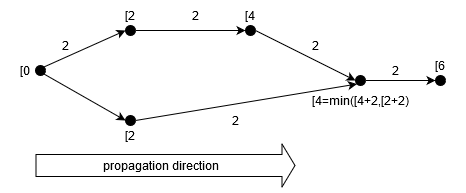
\includegraphics[width=0.8\textwidth]{H1_propagate_earliest.png}
	\caption{Illustration of $propagate\_earliest$ for an agent $a$ with speed $v(a)=\frac{1}{2}$ (i.e. $mrt=2$).}
	\label{fig:propagate_earliest}
\end{figure}


\begin{algorithm}
	\caption{$propagate\_latest$} \label{algo:propagate_latest}
	\begin{algorithmic}[1]
	    \Require $l$, $(S,L)$, $F$, $mrt$  s.t. $F\subseteq \dom(l)$
	    \Ensure $l$
	    \State $Open \leftarrow F$
	    \For {$v \in Open$}
    	    \For {$v^\prime \in S-F: (v^\prime,v) \in L$}
    	        \If{$v^\prime \not\in \dom(l)$}
    	            \State $l(v^\prime) \leftarrow -\infty$
    	        \EndIf
    			\State $l(v) \leftarrow \max \Set*{l(v^\prime), l(v)-mrt}$
    			\State $Open \leftarrow Open \cup \Set*{v^\prime}$
    		\EndFor
			\State $Open \leftarrow Open - \Set*{v}$
		\EndFor
	\end{algorithmic} 
\end{algorithm}


\begin{figure}[hbtp]
	\centering
  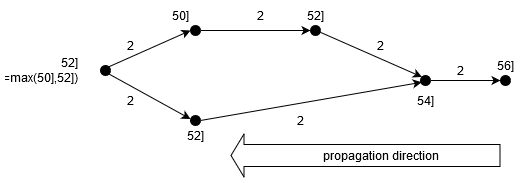
\includegraphics[width=0.8\textwidth]{H1_propagate_latest.png}
	\caption{Illustration of $propagate\_latest$ for an agent $a$ with speed $v(a)=\frac{1}{2}$ (i.e. $mrt=2$) and for upper bound $U=56$.}
	\label{fig:propagate_latest}
\end{figure}





For schedule generation, we use a different objective function than for re-scheduling, namely minimizing
\begin{equation}
\sum_{a \in \mathcal{A}, v,v^\prime \in P(a), in(v)=0, out(v^\prime)=0} A(a,v^\prime) - A(a,v)    
\end{equation}
and restricting
\begin{equation}
\max_{a \in \mathcal{A}, v \in P(a)} A(a,v) \leq U,
\end{equation}
where we use the following heuristic for the upper bound,
\begin{equation}
U=\delta \cdot  \left(w + h + \frac{\left|\mathcal{A}\right|}{\left| S \right|} \right)
\end{equation}
and $\delta=8$,
to find a schedule $S$ for a given service intention. This objective function is intended to mimick a green wave behaviour of real-world train scheduling (schedules are constructed such that there are only planned stops for passenger boarding and alighting); however, this also keeps us from introducing time reserves in the schedule and trains will not be able to catch up in our synthetic world.

Furthermore, we only use the shortest path for each agent for scheduling in order to speed-up schedule generation; if the upper bound $U$ is chosen liberal enough, then a solution is found where no train stops during its run.


Notice that trains have no length in the model: an edge is exited when the next edge is entered, but remains blocked for $r$ time steps after exit. Train extension can be introduced into this model by requiring consecutive edges to require the same resource; this again highlights that edges in the general train scheduling problem do not represent physical track sections; physical track sections have to be represented by resources.




%%%%%%%%%%%%%%%%%%%%%%%%%%%%%%%%%%%%%%%%%%%%%%%%%%%%%%%%%%%%%%%%%%%%%%%%%%
\subsection{Malfunction Generation}\label{subsubsec:malfunctiongeneration}
%%%%%%%%%%%%%%%%%%%%%%%%%%%%%%%%%%%%%%%%%%%%%%%%%%%%%%%%%%%%%%%%%%%%%%%%%%

Our experiment parameters contain the following parameters for malfunction generation:
\begin{itemize}
    \item $m_{earliest} \in \mathbb{N}$: the earliest time step the malfunction can happen after the scheduled departure;
    \item $m_{duration} \in \mathbb{N}$: how much the train will be delayed;
    \item $m_{agent} \in \mathcal{A}$: the train that is concerned.
\end{itemize}

Given the schedule, we derive our malfunction $M=(m_{time\_step},m_{duration},m_{agent})$ where
\begin{equation*}
m_{time\_step} = \min \left\{  A(m_{agent},\sigma(a, P)) + m_{earliest},  A(m_{agent},\tau(a,P) \right\},
\end{equation*}
which ensures that the agent malfunction happens while the train is running.




%%%%%%%%%%%%%%%%%%%%%%%%%%%%%%%%%%%%%%%%%%%%%%%%%%%%%%%%%%%%%%%%%%%%%%%%%%
\subsection{Objective for Re-Scheduling}
%%%%%%%%%%%%%%%%%%%%%%%%%%%%%%%%%%%%%%%%%%%%%%%%%%%%%%%%%%%%%%%%%%%%%%%%%%
We chose to to minimize a linear combination of delay with respect to the initial schedule $S0$ and penalizing diverging route segments (only the first edge of each such segment). This reflects the idea of not re-routing trains without the need of avoiding delay; if re-scheduling is applied in an iterative loop, this should help to avoid ``flickering'' of decisions.
%
Formally, the objective is to minimize over solutions $S=(P_S,A_S)$  the sum
\begin{equation}
\sum_{a \in \mathcal{A}} \delta\left(S(a,\tau(a,S)) - S0(a,\tau(a, S0))\right) + \rho \cdot \left|\left\{v \in \mathcal{V}(S,a)-\mathcal{V}(S0,a): (v^\prime,v) \in P_{S0}(a) \right\}\right| \label{eq:objectiveresched}
\end{equation}
where the \emph{delay model} is step-wise linear,
\begin{equation}
\delta(t) =
\begin{cases}
    \infty & \textrm{ if } t \geq \delta_{cutoff},\\
    \floor{t / \delta_{step}} \cdot \delta_{penalty}  & \textrm{else},
\end{cases}
\end{equation}
for hyper-parameters $\delta_{step}$, $\delta_{cutoff}, \delta_{penalty}$
and the second term of (\ref{eq:objectiveresched}) penalizes re-routing with respect to the initial schedule S0 by weight $\rho$ for every first edge deviating from the original schedule $S0$ .


%%%%%%%%%%%%%%%%%%%%%%%%%%%%%%%%%%%%%%%%%%%%%%%%%%%%%%%%%%%%%%%%%%%%%%%%%%
\subsection{Re-Scheduling Scopes}
%%%%%%%%%%%%%%%%%%%%%%%%%%%%%%%%%%%%%%%%%%%%%%%%%%%%%%%%%%%%%%%%%%%%%%%%%%



%%%%%%%%%%%%%%%%%%%%%%%%%%%%%%%%%%%%%%%%%%%%%%%%%%%%%%%%%%%%%%%%%%%%%%%%%%
\subsubsection{(Empty) Scoping Re-scheduling (full after malfunction)}\label{subsubsec:Delta0}
%%%%%%%%%%%%%%%%%%%%%%%%%%%%%%%%%%%%%%%%%%%%%%%%%%%%%%%%%%%%%%%%%%%%%%%%%%


We first describe full the re-scheduling problem as a general train scheduling problem. Let $N=(V,E,R,m,a,b)$ be the network of train scheduling problem, $(P,A)$ be a solution to it and let $M=(m_{time\_step},m_{duration},m_{agent})$ be a malfunction.

Informally, the \emph{re-scheduling problem} is the train scheduling problem such that
\begin{itemize}
    \item all decisions up to and including $m_{time\_step}$ are fixed from the solution. If the train is on an edge at $m_{time\_step}$, then it has to use the same edge, reflecting that a train on a straight segment has to continue and the switch position cannot be changed once the train is on the switch;
    \item the train corresponding to $m_{agent}$ is delayed by $m_{duration}$.
\end{itemize}
We here have two options:
\begin{enumerate}
    \item we can constrain the original scheduling up to the malfunction
    \item we can remove everything up to the malfunction and constrain only the last decision before the malfunction
\end{enumerate}
In order to keep the exposition simple and since this is also in the spirit of a re-scheduling loop with moving time horizon, we adopt the second option in the following exposition.\footnote{The implementation follows option 1. Should we adapt the implementation?}



We now describe the transformations $\Delta_0$ for a single train in Algorithm~\ref{algo:Delta0}:
If the train is already done at the malfunction time step, it can be removed from the problem; 
if the train has not started yet at the malfunction time step, we keep its start node fixed from $S0$ and do not start earlier than in $S0$ and use $propagate$ (described below) to derive the constraints. 




\begin{mdframed}
{\bf TODO Christian} in case 2 (not started yet), we should respect the malfunction delay? Problem here and in source code!
\end{mdframed}




\begin{algorithm}
	\caption{$Delta_0$ for train $a$} \label{algo:Delta0}
	\begin{algorithmic}[1]
		\Require $(S,L)$, $(P,A)$, $M=(m_{time\_step},m_{duration},m_{agent})$, mrt, U, c
	    \Ensure $(S,L),e,l$
        \If{$\max_{v\in S} A(v) \leq m_{time\_step}$}
            \State $S\leftarrow \emptyset$, $L \leftarrow \emptyset$
        \ElsIf{$\min_{v\in S} A(v) > m_{time\_step}$}
            \State $v_1 \leftarrow \argmin_{v\in S} A(v)$
            \State $e(v_1) \leftarrow A(v_1)$
            \For{$\tau \in S: out(\tau)=0$}
                \State $l(\tau)=U$ 
            \EndFor
            \State $F_v \leftarrow F_e \leftarrow \Set*{v_1}$
            \State $F_l \leftarrow \Set*{\tau \in S: out(\tau)=0}$
            \State $e,l,(S,L) \leftarrow propagate(e,l,(S,L),F_e,F_l,F_v, mrt, U, c)$
        \Else
            \State $e,l,(S,L) \leftarrow Delta\_0\_running((S,L), (P,A), M, mrt, U, c)$
        \EndIf
\end{algorithmic} 
\end{algorithm}


Before describing the third case of the malfunction happening while the train is running, we describe \emph{propagate} (Algorithm~\ref{algo:propagate}): We first propagate earliest and latest, then truncate time windows to $c$; we need to propagate latest again since truncation might spoil the semantics of $l(v)$ being the latest possible passing time to reach the target in time. Finally, we remove nodes that are not reachable in time (because of an empty time window) or cannot be reached from one of the nodes $F_v$ that must be visited.

\begin{algorithm}
	\caption{$propagate$} \label{algo:propagate}
	\begin{algorithmic}[1]
	    \Require $e,l,(S,L),F_e,F_l,F_v,mrt,U,c$ 
	    \Ensure $e,l,(S,L)$
        \For{$v \in F_v$}
		    \State $S \leftarrow \Set{v^\prime \in S: \textrm{there is a }v\textrm{--}v^\prime\textrm{ path or a }v^\prime\textrm{--}v\textrm{ path in }L}$
		    \State $L \leftarrow \Set*{(v,v^\prime) \in L: v,v^\prime \in S}$
		\EndFor
	    \State $e \leftarrow propagate\_earliest(e, (S,L), F_e, mrt)$
		\State $l \leftarrow propagate\_latest(l,(S,L),F_l, mrt)$
		\If{$c < \infty$}
		\For{$v\in S-F_e$}
	        \State $l(v) \leftarrow \min \Set*{l(v), e(v)+c}$
	    \EndFor
	    \State $l \leftarrow propagate\_latest(l,(S,L),F_l, mrt)$
	    \EndIf
		\State $S \leftarrow \Set{v \in S: e(v) \leq l(v)}$, $L \leftarrow \Set*{(v,v^\prime) \in L: v,v^\prime \in S}$

	\end{algorithmic} 
\end{algorithm}



We now describe the remaining case of Algorithm~\ref{algo:Delta0}, namely when the malfunction happens while the train is running. We refer to Algorithm~\ref{algo:Delta0running}: we first determine the edge $(v_1,v_2)$ the train is on when the malfunction happens; we then fix the time for $v_1$ as in $S0$ and set the earliest for $v_2$, possibly delayed. Then, we use $propagate$ to tighten the search space. Notice that $propagate$ will here remove the nodes on the scheduled path before $v_1$ (since the forward propagation will not reach these nodes, they will be removed as the time window will be empty).


\begin{algorithm}
	\caption{$Delta\_0\_running$ for running train $a$} \label{algo:Delta0running}
	\begin{algorithmic}[1]
		\Require $(S,L)$, $(P,A)$, $M=(m_{time\_step},m_{duration},m_{agent})$, mrt, U, c
	    \Ensure $e,l,(S,L)$
	    \State $(v_1,v_2) \leftarrow (v_1,v_2) \in L$ s.t. $A(v_1)\leq m_{time\_step}$ and $A(v_2)>m_{time\_step}$
		\State $e(v_1)\leftarrow A(v_1)$, $l(v_1) \leftarrow A(v_1)$ 
        \If{$a$ corresponds to $m_{agent}$}
            \State $e_1(v_2) \leftarrow A(v_1)+mrt+m_{duration}$
        \Else
            \State $e_1(v_2) \leftarrow A(v_1)+mrt$
        \EndIf
        \State $F_e \leftarrow \Set*{v_1,v_2}$, $F_l \leftarrow \Set*{v_1} \cup \Set*{\tau \in S: out(\tau)=0}$
	
	    \For{$\tau \in S-\Set*{v_1}: out(\tau)=0$}
	        \State $l(\tau) \leftarrow U$
	    \EndFor
		\State $e,l,(S,L) \leftarrow propagate(e,l,(S,L),F_e,F_l, \Set*{v_1,v_2}, mrt, U, c)$
	\end{algorithmic} 
\end{algorithm}





        

%%%%%%%%%%%%%%%%%%%%%%%%%%%%%%%%%%%%%%%%%%%%%%%%%%%%%%%%%%%%%%%%%%%%%%%%%%
\subsubsection{Re-scheduling (delta perfect after malfunction)}\label{subsubsec:Deltaperfect}
%%%%%%%%%%%%%%%%%%%%%%%%%%%%%%%%%%%%%%%%%%%%%%%%%%%%%%%%%%%%%%%%%%%%%%%%%%

Now we define the perfect oracle as outlined above.
Let $(P_{S0},A_{S0})$ be the solution to the original train scheduling problem
and let $N_S=(V_S,E_S,R_S,m_S,a_S,b_S)$ be the network of the re-scheduling problem for an agent
and  let $(P_S,A_S)$ be a solution to the re-scheduling problem. Algorithm~\ref{algo:Deltaperfect} defines the perfect oracle: we keep fixed all times and nodes that are common to $S_0$ and $S$, respectively. Everything that is not reachable in path ($F=\Delta_P$) or time ($F_e=F_l=\Delta_A)$) will be removed by $propagate$. Notice that we have $v_1 \in\subseteq \Delta_A \subseteq \Delta_P$ and $v_2 \in \Delta_P$








\begin{mdframed}
{\bf TODO Christian} does $Delta_{perfect}$ work if the agent has already terminated or has not started at malfunction time?
\end{mdframed}


\begin{algorithm}
	\caption{$Delta_{perfect}$} \label{algo:Deltaperfect}
	\begin{algorithmic}[1]
		\Require $(S,L)$, $(P_{S_0},A_{S_0})$, $(P_S,A_S)$, $M=(m_{time\_step},m_{duration},m_{agent})$, mrt, U, c
	    \Ensure $e,l,(S_1,L_1)$
	    \State $\Delta_A \leftarrow \Set*{v: A_S(v)=A_{S_0}(v)}$
	    \State $\Delta_P \leftarrow \Set*{v: v\in P_S, v\in P_{S_0}}$
	    \State $S_1 \leftarrow \Set*{v: v\in P_{S_0}} \cup \Set*{v: v\in P_{S}}$
	    \State $L_1 \leftarrow \Set*{(v,v^\prime) \in P_S \textrm{ or } (v,v^\prime) \in P_{S_0}: v,v^\prime \in S_1}$
	    \For {$v \in \Delta_A$}
	        \State $l(v)\leftarrow e(v)\leftarrow A_{S_0}(v)$
	    \EndFor
	    \For{$v \in S_1-\Delta_A: out(v)=0$}
	        \State $l(v) \leftarrow U$
	    \EndFor
	    \State $(v_1,v_2) \leftarrow (v_1,v_2) \in L_1$ s.t. $A_{S_0}(v_1)\leq m_{time\_step}$ and $A_{S_0}(v_2)>m_{time\_step}$
	    \If{$v_2 \not \in \Delta_A$}
        \If{$a$ corresponds to $m_{agent}$}
            \State $e_1(v_2) \leftarrow A_{S_0}(v_1)+mrt+m_{duration}$
        \Else
            \State $e_1(v_2) \leftarrow A_{S_0}(v_1)+mrt$
        \EndIf
        \EndIf
	    \State $e,l,(S_1,L_1) \leftarrow propagate(e,l,(S_1,L_1),\Delta_A \cup \Set*{v_2}, \Delta_A, \Delta_P, mrt, U, c)$
	\end{algorithmic} 
\end{algorithm}

\begin{mdframed}
{\bf TODO Christian}
Formalize Delta\_0/Delta\_perfect of the whole problem for all agents. 
Proposition: "Delta\_perfect <= Delta\_0", i.e. every solution to Delta\_perfect is a solution to Delta\_0
\end{mdframed}


%%%%%%%%%%%%%%%%%%%%%%%%%%%%%%%%%%%%%%%%%%%%%%%%%%%%%%%%%%%%%%%%%%%%%%%%%%
\subsubsection{Naive Re-scheduling (delta naive after malfunction)}\label{subsubsec:Deltanaive}
%%%%%%%%%%%%%%%%%%%%%%%%%%%%%%%%%%%%%%%%%%%%%%%%%%%%%%%%%%%%%%%%%%%%%%%%%%

\begin{mdframed}
{\bf TODO Christian} pseudo-code naive prediction
\end{mdframed}


%%%%%%%%%%%%%%%%%%%%%%%%%%%%%%%%%%%%%%%%%%%%%%%%%%%%%%%%%%%%%%%%%%%%%%%%%%
\subsubsection{Online Re-scheduling (delta online after malfunction)}\label{subsubsec:Deltaonline}
%%%%%%%%%%%%%%%%%%%%%%%%%%%%%%%%%%%%%%%%%%%%%%%%%%%%%%%%%%%%%%%%%%%%%%%%%%




\begin{mdframed}
{\bf TODO Christian} a bit of introduction after all...
\end{mdframed}


\begin{algorithm}
	\caption{$transmissionchains$} \label{algo:naive}
	\begin{algorithmic}[1]
		\Require $\mathcal{A}$, $(P_S,A_S)$, $\mathcal{A}^*\subseteq\mathcal{A}$
	    \Ensure $\mathcal{A}$
	    % not-changed agents
	    \For {$(S,L,e,l,w) \in \mathcal{A}-\mathcal{A}^*$}
	        \State $S \leftarrow \Set*{v: v\in P_{S}}$
	        \State $L \leftarrow \Set*{(v,v^\prime) \in P_{S}: v,v^\prime \in S_1}$
	        \State $e \leftarrow \Set*{(v,P_S(v): v\in S}$
	        \State $l \leftarrow \Set*{(v,P_S(v): v\in S}$
	        \State $w \leftarrow w \vert_{L}$
	    \EndFor
	\end{algorithmic} 
\end{algorithm}


Reduce the strictness of the oracle by freeing up all the variables of changed trains. I.e. if a train has some change somewhere, all the parameters of the train are available or change such as alternative routes and different times. This is detailled in Algorithm~\ref{algo:DeltaNotperfect}, where $\mathcal{A}^*$ denotes the set of changed trains and $\mathcal{A}$ are the trains as of the full re-scheduling problem.


\begin{algorithm}
	\caption{$Delta_{notsoperfect}$} \label{algo:DeltaNotperfect}
	\begin{algorithmic}[1]
		\Require $\mathcal{A}$, $(P_S,A_S)$, $\mathcal{A}^*\subseteq\mathcal{A}$
	    \Ensure $\mathcal{A}$
	    % not-changed agents
	    \For {$(S,L,e,l,w) \in \mathcal{A}-\mathcal{A}^*$}
	        \State $S \leftarrow \Set*{v: v\in P_{S}}$
	        \State $L \leftarrow \Set*{(v,v^\prime) \in P_{S}: v,v^\prime \in S_1}$
	        \State $e \leftarrow \Set*{(v,P_S(v): v\in S}$
	        \State $l \leftarrow \Set*{(v,P_S(v): v\in S}$
	        \State $w \leftarrow w \vert_{L}$
	    \EndFor
	\end{algorithmic} 
\end{algorithm}



%%%%%%%%%%%%%%%%%%%%%%%%%%%%%%%%%%%%%%%%%%%%%%%%%%%%%%%%%%%%%%%%%%%%%%%%%%
\subsubsection{Random Online Re-scheduling (delta random after malfunction)}\label{subsubsec:Deltarandom}
%%%%%%%%%%%%%%%%%%%%%%%%%%%%%%%%%%%%%%%%%%%%%%%%%%%%%%%%%%%%%%%%%%%%%%%%%%
        
\begin{mdframed}
{\bf TODO Christian} a bit of introduction after all...

% random as a naive baseline from those running after the malfunction → if that also reduces solution time, our problem is not hard enough, showing the problem is not trivia

%     total_changed = wieviele Agenten haben wirklich geändert?
%         free up malfunction agent + total_changed - 1 random agenten (active or future active)
%         (Warnung) Achtung time window muss gross sein
%         Nur für ausgewählte Experimente?
%     total_changed = wieviele Agenten haben im Online geändert?
\end{mdframed}

        
%%%%%%%%%%%%%%%%%%%%%%%%%%%%%%%%%%%%%%%%%%%%%%%%%%%%%%%%%%%%%%%%%%%%%%%%%%
%%%%%%%%%%%%%%%%%%%%%%%%%%%%%%%%%%%%%%%%%%%%%%%%%%%%%%%%%%%%%%%%%%%%%%%%%%
\section{Computational Results}\label{sec:Results}
%%%%%%%%%%%%%%%%%%%%%%%%%%%%%%%%%%%%%%%%%%%%%%%%%%%%%%%%%%%%%%%%%%%%%%%%%%
%%%%%%%%%%%%%%%%%%%%%%%%%%%%%%%%%%%%%%%%%%%%%%%%%%%%%%%%%%%%%%%%%%%%%%%%%%




%%%%%%%%%%%%%%%%%%%%%%%%%%%%%%%%%%%%%%%%%%%%%%%%%%%%%%%%%%%%%%%%%%%%%%%%%%
\subsection{Experiment Design}
%%%%%%%%%%%%%%%%%%%%%%%%%%%%%%%%%%%%%%%%%%%%%%%%%%%%%%%%%%%%%%%%%%%%%%%%%%

In light of the findings of the previous paragraphs, we design our experiments in a hierarchical fashion on multiple levels
\begin{enumerate}
    \item infrastructure
    \item schedule
    \item malfunction
    \item solver runs
\end{enumerate}
where at each level we generate multiple instances for a fixed instance of the previous levels (i.e. we generate multiple infrastructures for the same parameters, we generate multiple schedules for the same infrastructure etc.). The lowest level is a sanity level to investigate the variance of the solver for the same problem.

The agenda for the results of this section is shown in Figure~\ref{fig:agenda}: We have
\begin{itemize}
    \item 8 infrastructures with 80 to 150 agents (i.e. the first infrastructure has 80 agents, the second has 88 agents)
    \item 10 schedules per infrastructure
    \item for every agent a malfunction 30 time steps after its scheduled start for 50 time steps
    \item 1 solver run
\end{itemize}
This gives an agenda of 8640 experiments.
The data is available in a dedicated git repository \url{https://github.com/SchweizerischeBundesbahnen/rsp-data}.
%
Infrastructure, schedule and the experiment results shown in this section are in
\textrm{h1\_2020\_08\_24T21\_04\_42/h1\_2020\_08\_24T21\_04\_42\_baseline\_2020\_09\_17T17\_08\_13}; in these provisional results, only the first 803 experiments have been run. 

\begin{mdframed}
{\bf TODO Christian} Run and upload full agenda, finalize
\end{mdframed}


We filter out  experiments with small absolute and large relative run times:
\begin{itemize}
    \item time full after malfunction $< 10$s
    \item time full after malfunction $> 97\%$-percentile of time full after malfunction
\end{itemize}
This filters out 25 experiments and leaves us with data from 778 experiments.


\begin{figure}[hbtp]
	
    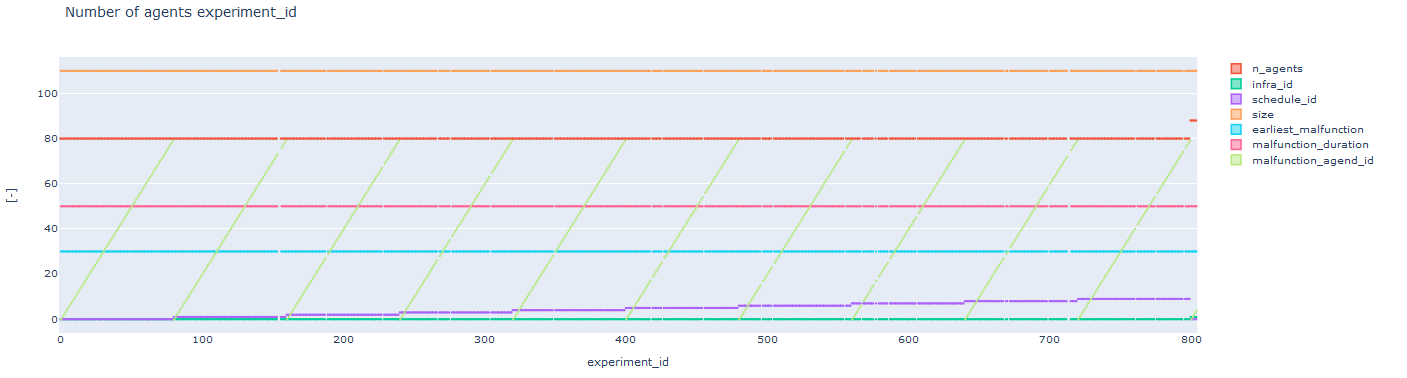
\includegraphics[width=\textwidth]{Figures/agenda.PNG}
	\caption{Hierarchical Agenda Structure.}
	\label{fig:agenda}
\end{figure}




%%%%%%%%%%%%%%%%%%%%%%%%%%%%%%%%%%%%%%%%%%%%%%%%%%%%%%%%%%%%%%%%%%%%%%%%%%
\subsection{Speed-Up and Solution Quality}
%%%%%%%%%%%%%%%%%%%%%%%%%%%%%%%%%%%%%%%%%%%%%%%%%%%%%%%%%%%%%%%%%%%%%%%%%%

\begin{figure}[hbtp]
    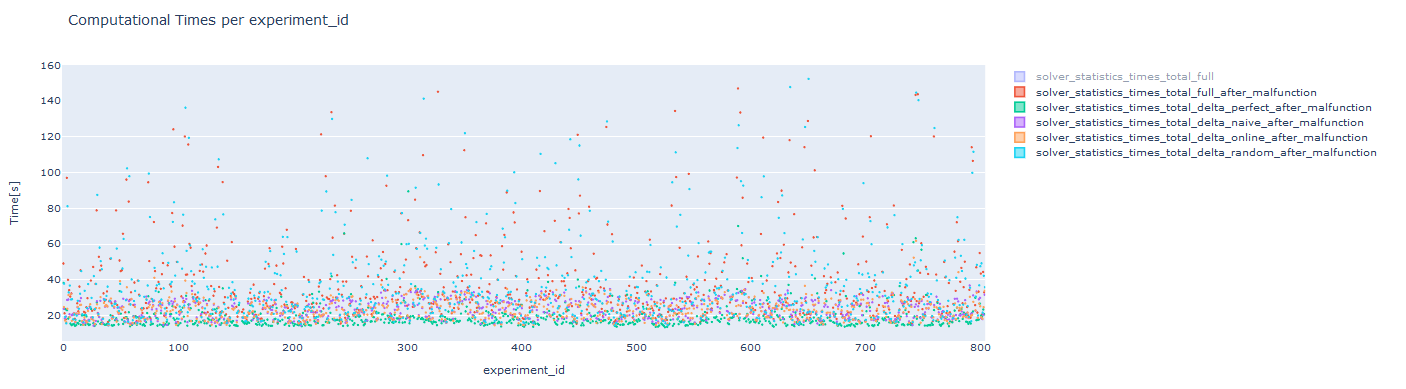
\includegraphics[width=\textwidth]{Figures/computation_times_per_experiment_id.PNG}
	\caption{Computation times per experiment.}
	\label{fig:computationtimesexperimentid}
\end{figure}
In Figure~\ref{fig:computationtimesexperimentid}, we do no recognize any block structure of running times as we could expect from Figure~\ref{fig:agenda}. In other words, grid size and number of against is not a good measure of the difficulty of the re-scheduling problem (we conjecture that it may be even hard to determine beforehand whether a problem is hard); furthermore, the difficulty varies greatly for the same schedule when taking different agents (notice that this implies different time steps as well since the malfunction is performed 30 time steps after the malfunction agent's departure). We will come back to this in Section~\ref{sec:CaseStudies}, where we give some illustrations.

Therefore, we trivially take the full re-scheduling time as measure of problem complexity and plot the rescheduling times and speed-up for the different scopes against the full re-scheduling time in Figure~\ref{fig:computationtimes}
We see a clear speed-up for almost all experiments except for the random scoper, which is reflected by the random scope has runtimes staying along the diagonal (full rescheduling time) and speed-up being around $1.0$.
Furthermore, the re-scheduling times for more difficult problems in the reduced scopes (delta perfect, delta naive, delta online) seem to stay in an almost constant range; this is reflected by an increasing speed-up with respect to the full re-scheduling time.

With these preliminary results, do not see a clear separation between the scopes, only a slight tendency for the speed-up being greatest in delta perfect.



\begin{figure}[hbtp]
	
    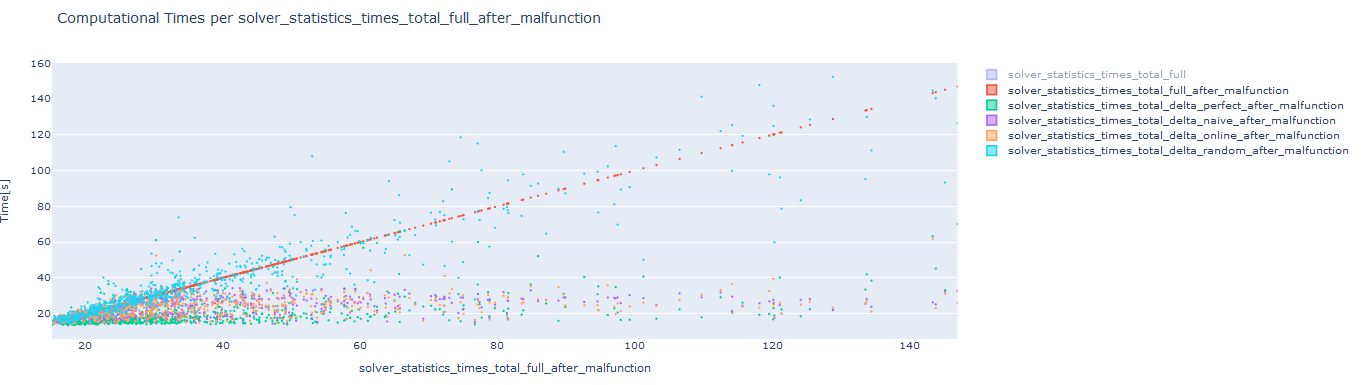
\includegraphics[width=\textwidth]{Figures/computation_times_per_times_total_full_after_malfunction.PNG}
        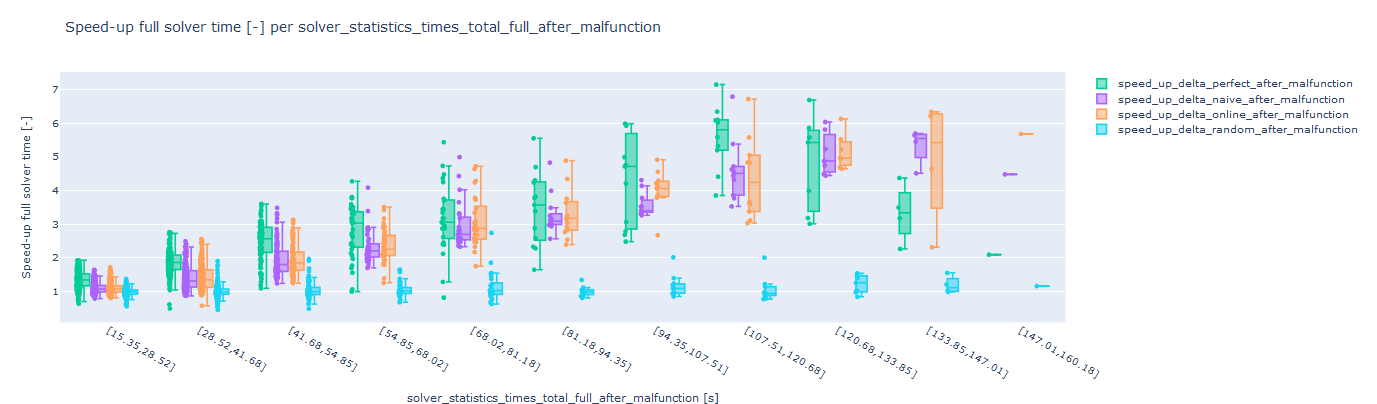
\includegraphics[width=\textwidth]{Figures/speedup.PNG}
	\caption{Re-scheduling times and speed-up against full re-scheduling time. The speed-ups are grouped in 10 bins of equal size on the horizontal axis between min and max value.}
	\label{fig:computationtimes}
\end{figure}

\begin{mdframed}
{\bf TODO Christian} visualize effective costs and ratio: delta perfect and delta naive should reach same costs 
\end{mdframed}

\begin{figure}[hbtp]
    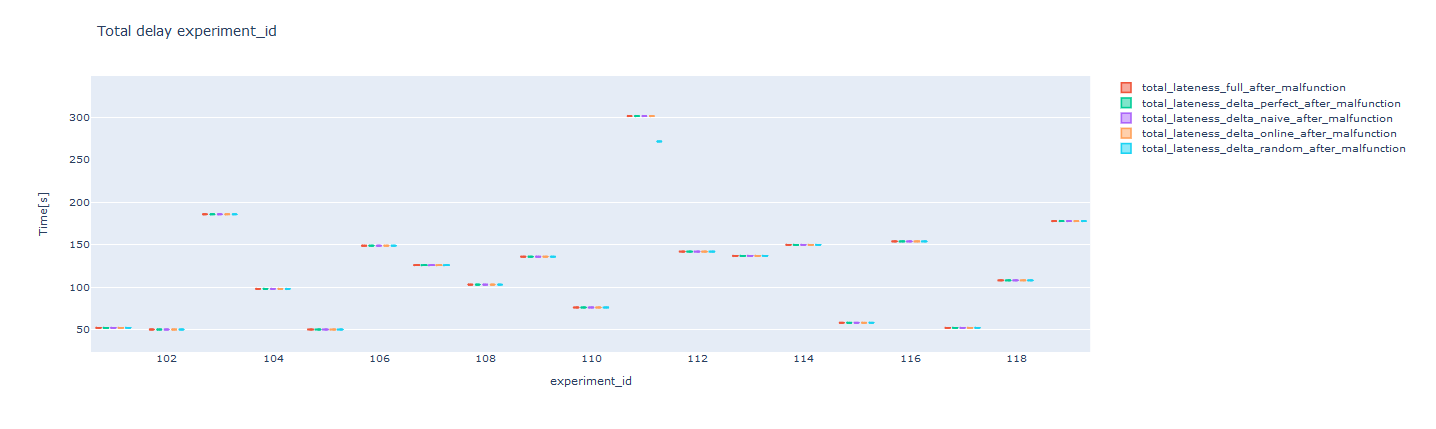
\includegraphics[width=\textwidth]{Figures/total_delay.PNG}
	\caption{.}
	\label{fig:delay}
\end{figure}


%%%%%%%%%%%%%%%%%%%%%%%%%%%%%%%%%%%%%%%%%%%%%%%%%%%%%%%%%%%%%%%%%%%%%%%%%%
\subsection{Prediction Quality of Online Scopes}
%%%%%%%%%%%%%%%%%%%%%%%%%%%%%%%%%%%%%%%%%%%%%%%%%%%%%%%%%%%%%%%%%%%%%%%%%%

\begin{mdframed}
{\bf TODO Christian} false positives, false negatives etc.
\end{mdframed}

%%%%%%%%%%%%%%%%%%%%%%%%%%%%%%%%%%%%%%%%%%%%%%%%%%%%%%%%%%%%%%%%%%%%%%%%%%
\subsection{Model Calibration}
%%%%%%%%%%%%%%%%%%%%%%%%%%%%%%%%%%%%%%%%%%%%%%%%%%%%%%%%%%%%%%%%%%%%%%%%%%

\begin{mdframed}
{\bf TODO Christian} ASP: preprocessing vs. solving; different parameters (delay model?): which parameters make the problem harder, what do we measure?
\end{mdframed}


%%%%%%%%%%%%%%%%%%%%%%%%%%%%%%%%%%%%%%%%%%%%%%%%%%%%%%%%%%%%%%%%%%%%%%%%%%
%%%%%%%%%%%%%%%%%%%%%%%%%%%%%%%%%%%%%%%%%%%%%%%%%%%%%%%%%%%%%%%%%%%%%%%%%%
\section{Case Studies}\label{sec:CaseStudies}
%%%%%%%%%%%%%%%%%%%%%%%%%%%%%%%%%%%%%%%%%%%%%%%%%%%%%%%%%%%%%%%%%%%%%%%%%%
%%%%%%%%%%%%%%%%%%%%%%%%%%%%%%%%%%%%%%%%%%%%%%%%%%%%%%%%%%%%%%%%%%%%%%%%%%

\begin{mdframed}
{\bf TODO Christian} example of cost-equivalent solutions; example of false negative, false positive; malfunction variation
\end{mdframed}


%%%%%%%%%%%%%%%%%%%%%%%%%%%%%%%%%%%%%%%%%%%%%%%%%%%%%%%%%%%%%%%%%%%%%%%%%%
%%%%%%%%%%%%%%%%%%%%%%%%%%%%%%%%%%%%%%%%%%%%%%%%%%%%%%%%%%%%%%%%%%%%%%%%%%
\section{Extended Discussion/Related Work/Literature: show links to various Research Approaches}
%%%%%%%%%%%%%%%%%%%%%%%%%%%%%%%%%%%%%%%%%%%%%%%%%%%%%%%%%%%%%%%%%%%%%%%%%%
%%%%%%%%%%%%%%%%%%%%%%%%%%%%%%%%%%%%%%%%%%%%%%%%%%%%%%%%%%%%%%%%%%%%%%%%%%

\begin{mdframed}
{\bf TODO Emma}         ML
        delay propagation / recourse / stability of iterative and batch processing
        simulation
        OR / heuristics (job insertion)
        decomposition approaches
        real-time rescheduling
        
\end{mdframed}        

\bibliographystyle{unsrt}
\bibliography{biblio}

\end{document}






\section{Introduction}
Here we describe the Re-Scheduling problem.

Switzerland has a dense railway network with both freight and passenger trains running on the same infrastructure. More than 1.2 million people use trains on a daily basis. In Railway Operations, the operational schedule has to be continually re-computed because of many smaller and larger delays that arise during operations. Not all of those can be absorbed by extra times in the schedule, and if the delay has an impact on other trains, decisions on re-ordering or re-routing trains have to be taken to derive a new feasible operational plan. The industry state of the art is that delay propagation is efficiently re-computed by online IT systems. Conflicts, however, have to be most often resolved by humans by explicitly deciding on re-ordering or re-routing based on their experience. Because of the massive combinatorial complexity of these microscopic models, Operations Research models are currently only applied in very restricted, highly condensed areas for re-ordering decisions and only very limited routing alternatives, if any.
Research Approach

To tackle this problem, our approach is to combine Operations Research and Machine Learning to get the best of both worlds: a Graph Neural Network acts as an Oracle for Operations Research by learning a heuristic that predicts the "impact" of a delay; we hope the Oracle could predict which trains and which departures are or could be affected by the delay based on past decisions. This piece of information from the oracle then helps the (MILP or CP) solver to constrain the search space or at least drive its search more efficiently (driving the branching process). We hope that Graph Neural Networks are a natural way to represent the graph structure of railway networks.

Our considerations are based on the Re-Scheduling Effects Model of Figure~\ref{fig:EffectsModel}:
the Operational Schedule is based on being informed about delays and the schedule communicated to customers. Interventions may be redefine the allowed speeds per location or per train, the available routes, the connections to be kept or dropped and trains to be added or dropped. Interventions may be directly based on events happening in reality or based on the current network status aggregated from past events. 
%
Events from reality are interpreted when lead to a difference to the Operational Schedule.
%
\begin{figure}[hbtp]
	\centering
  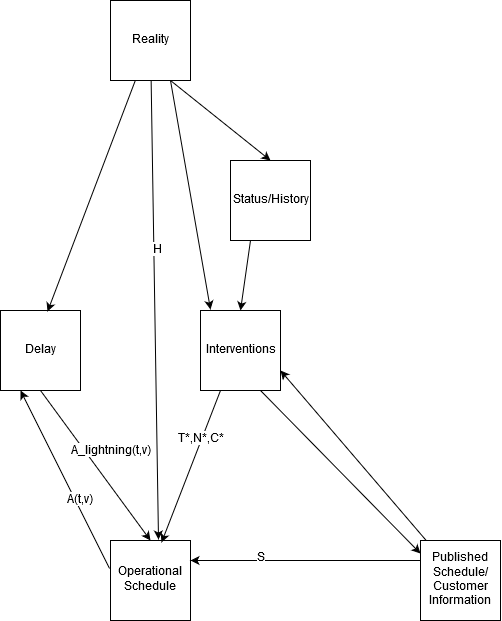
\includegraphics[width=0.7\textwidth]{Wirkungsmodell.png}
	\caption{Re-Scheduling Effects Model. Arrows represent logical dependencies. The symbols on the arrows are those used in the formal problem description later on.}
	\label{fig:EffectsModel}
\end{figure}
\section{Related Work}

TODO Related Work. How does it relate to \cite{DBLP:journals/corr/abs-1807-11876}?
TODO Other different approaches: Benders-like decomposition and loop, generate-and-verify-loop


\section{Methodology}
Here we describe the three hypotheses and the pipeline.

\subsection{3 Hypotheses, one building on the previous}
\begin{description}
\item[Hypothesis 1] We can compute good recourse actions, i.e., an adapted plan within a small fraction of the full solution time if all variables are fixed, except those related to services that are affected by the disruption implicitly or explicitly.
\item[Hypothesis 2] Machine learning can predict services that are affected by disruptions implicitly or explicitly with respect to a fixed infrastructure and a fixed basic (published) schedule, without the intention of model training to generalize over infrastructures nor completely new timetable concepts.
\item[Hypothesis 3] If hypothesis 2 is true, in addition, machine learning can predict the state of the system in the next time period after re-scheduling.
\end{description}

\subsection{A General Framework}
Our approach can be seen as a general framework with the following ingredients:
\begin{description}
\item[Detailed Model] We have a model  that reflects the detailed  view but which cannot be applied because it would be intractable. A detailed model acts at the operational and could be produced in reality if no further delays or disruptions happen; it not only works at the more imprecise tactical level. Formally, the detailed model is a deterministic solver that produces an operational plan ${\bf y}^*({\bf x})$ for a problem ${\bf x}$.
\item[Oracle] An Oracle predicts relevant parts of the solution such that the detailed exact model becomes tractable if we complement it by the informed guess by the Oracle.
Formally, an Oracle ${\cal O}$ produces an enhanced input ${\cal O}({\bf x})$ such that ${\bf y}^*({\cal O}({\bf x}))$ can be computed more efficiently.
\item[Simulation] Verifying an Oracle in the real world is often too expensive, either in financial terms or because of legal or other risk issues. Simulation allows us to train and verify the Oracle without having to run those risks. More formally, a simulation produces realistic inputs ${\bf x}$ (following the same distribution).
\end{description}



\subsection{Pipeline for Verification of Hypothesis 1}
Input generation
Step
Generate infrastructure
Generate schedule
Generate disturbance
Full Schedule (w/o disturbance)
Hypothesis Validation

How big is the speed up if we know Delta?
Step
Re-Scheduling full w/o restrictions
Determine Delta w.r. to Full Schedule
Re-Scheduling Delta



\section{Formal Problem Definition}
\subsection{FLATland Formal Definition}
Gridworld and Semantics. I'd like to formalize this. I think it would be worth to describe the FLATland semantics (synchronization, entering Grid, malfunctions, speed model). This will help us to generalize/abstract.


\subsection{Scheduling Problem}
Our formulation is based on \cite{DBLP:conf/lpnmr/AbelsJOSTW19}, but we slightly modify it in order to make the equivalence of microscopic halting sections explicit in the mathematical formulation. We will need this explicit property in the definition the Re-Scheduling Problem.\footnote{TODO: consistency of connections is not enforced - do we need it?} The naming is based on \cite{crowdAISBB}.


A \emph{Scheduling Problem} is a triple $(N,T,C)$ consisting of 
\begin{itemize}
    \item a \emph{Railway Network} $N=(V,E,R,m,a,b)$ where
    \begin{itemize}
        \item \emph{global route graph} $(V,E)$, which  is a directed graph; the edges are also called \emph{route sections}
        \item $R$ is a set of resources
        \item \emph{minimum travel times} per route section $m: E \to \NNN$
        \item \emph{resource allocations} on route sections $a: R \to 2^E$
        \item \emph{blocking or release times} per resource $R\to \NNN$
        
    \end{itemize}
    \item \emph{trains} T of the form $T\ni t = (V^t,E^t,e^t, l^t,w^t)$ where
    \begin{itemize}
        \item \emph{route graph} $(V^t,E^t)$ is an acyclic sub-graph of $(V,E)$
        \item \emph{earliest passing time} of train $t$ at a vertex: $e^t: V^t \to \NNN$
        \item \emph{latest passing time} of train $t$ at a vertex $l^t: V^t \to \NNN$ 
        \item \emph{waiting times} of train $t$ on edge $w^t: E^t \to \NNN$
        \item a partition $W^t=\{W_1^t,\ldots,W_n^t\} \subseteq 2^{E^t}$ of equivalent microscopic edges such that every path  $p=(v_0,\ldots,v_k) \subseteq V^t$ for $(v_i,v_{i+1})\in E^t$ for $i=1,\ldots,n-1$ \footnote{We use the following notation: $(v_0,\ldots,v_n)\subseteq V^t$ denotes an ordered subset of elements of $V^t$. TODO: Should we formally introduced the set of paths in $V^t$, relating to $E^t$ to simplify notation?} such that $in(v_0)=0$ and $out(v_n)=0$ contains exactly one element of each partitioning element $W_i$, $i=1,...,n$ (i.e. there is exactly one edge $w(W_i^t)=(v_j,v_{j+1})\in E^t$ for $W_i^t \in W$ and  $v_j,v_{j+1}\in p$ and such that all $w(W_i^t)$ are different (i.e. $w$ is injective)).
    \end{itemize}
    \item \emph{connections} $C\subseteq T \times E \times T \times E \times \NNN$ such that $(t_1,e_1,t_2,e_2,c)\in C \implies e_1 \in E^{t_1}, e_2 \in E^{t_2}$
\end{itemize}
Note that $(V,E)$ needs not be connected, i.e. each train may have its own (disjoint) route sub-graph, which is linked to other trains' route graph only through shared resources in $R$, and the union of of all train-specific route graphs needs not cover $(V,E)$.
Notice that the some consistency conditions of the real-world problem are not part of this formal definition, for instance we would have to ensure that every path can produce the commercial stops on different platform tracks.

A solution $(P,A)$ of the Scheduling Problem consists of the 
\begin{itemize}
    \item the selected paths $P: T \to 2^V$ where $p(t)=(t_1,\ldots,t_n)\subseteq V^t$ (we use $\ell(p(t))=n$ for the length of the path) is an ordered set satisfying
        \begin{equation}
            (v_i, v_{i+1})\in E^t\textrm{  for }i\in\{1,\ldots,n-1\} \label{eq:path_consistency}
        \end{equation}
        \begin{equation}
            in(v_1)=0\textrm{ and } out(v_n)=0 \label{eq:start_and_target_node}
        \end{equation}
        where $in:V\to\NNN$ and $out:V\to\NNN$ associate in and out degrees of vertices.
    \item partial allocation $A: T\times V \to \NNN$ where $A(t,v)$ is defined for $v\in P(t)$ satisfying
        \begin{equation}
            A(t,v) \geq e^t(v)\textrm { for } v \in P(t) \label{eq:earliest_requirement}
        \end{equation}
        \begin{equation}
             A(t,v) \leq l^t(v)\textrm { for } v \in P(t) \label{eq:latest_requirement}\\
        \end{equation}
        \begin{equation}
             A(t,v_i) + m((v_i,v_{i+1}) + w^t((v_i,v_{i+1})) \leq A(t,v_{i+1}) \label{eq:minimum_running_time_requirement}
        \end{equation}
        \begin{eqnarray}
             A(t_1, v^\prime) +b(r)\leq A(t_2, u) \xor A(t_2, u^\prime) +b(r) \leq A(t_1, v) \nonumber\\
             \textrm { for } v,v^\prime in  \in P(t_1), u,u^\prime \in P(t_2), (v,v^\prime),(u,u^\prime)\in a(r)
             \label{eq:mutual_resource_allocation_requirement}
        \end{eqnarray}
        (where $\xor$ denotes exclusive or)
        \begin{equation}
             A(t_1, v) +c\leq A(t_2, u) \textrm{ for }(t_1,(v,v^\prime),t_2,(u,u^\prime),c) \in C\label{eq:connection_requirement}
        \end{equation}
\end{itemize}

\subsection{FLATland as Scheduling Problem}
How are the route graphs derived from FLATland in general?


\subsection{Commercial and Operational Schedule}
The result of the above (offline) Scheduling Approach is a conflict-free (microscopic) solution. We therefore call it an \emph{Operational Schedule}.
If everything runs smoothly, it contains all the information required to run trains.

What we publish to customers needs not be as details and may not even be conflict-free in the microscopic sense. For instance, we might publish two trains to start at the same time and decide online which one goes first whichever is ready first.
Formally, given an Operational Schedule $(P,A)$,
a \emph{Commercial or Published Schedule} captures the elements published to consumers\footnote{TODO: Should the connections be part of the Commercial Schedule as well?}. Formally,
\begin{itemize}
    \item $S(t,v)$ is the published schedule, partially defined for $v_{i+1} \in P(t)=(v_1,\ldots,v_n)$ where $w^t(v_i)>0$ and satisfying $S(t,v)\leq A(t,v)$ and $S(t,v_j) \leq S(t,v_k)$ for $j<k$ and $v_j,v_k \in P(t)$  
\end{itemize}
i.e. we allow for conflicts in the commercial schedule, but guarantee that we never depart earlier than published in $S$.



\subsection{Re-Scheduling Problem}
Given a 
\begin{itemize}
    \item Operational Schedule $(P,A)$,
    \item Commercial Schedule $S$
    \item the current time $H \in \NNN$
    \item operational interventions in the form of a scheduling problem $(N^*,T^*, C^*)$
    \item an event $A^\lightning(t^\lightning,v^\lightning)\geq H$, $A^\lightning(t,v)\not=A^(t,v)$, $A(t,v) \geq H$
\end{itemize}
The interpretation of $H$ is that we have received all information up to $H$, i.e. all times  $A(v,t) \leq H$ are fixed, i.e. they are already included included in our current operational schedule (either because they worked according to our initial plan or because we have already updated our current operational schedule). We require $A^\lightning(t,v) \geq H$; the interpretation is that $A^\lightning(t^t\lightning,v^\lightning)$ is a prognosis when train $t$ will pass at $v$ for $A(t,v)\geq H$. 
Examples:
\begin{itemize}
    \item If $A^\lightning(t^\lightning,v^\lightning)=H$ and we know that we will be ready only later on at $A^\lightning(t^\lightning,v^\lightning)\not=A^(t^\lightning,v^\lightning)$, $A(t,v) \geq H$.
    \item If $A(t^\lightning,v^\lightning)>H$, we might know that we will be ready earlier at $A^\lightning(t^\lightning,v^\lightning) < A(t^\lightning,v^\lightning)$
\end{itemize}
A \emph{Re-Scheduling Oracle} is a pair $(F_1,F_2)$
\begin{itemize}
    \item $F_1\subseteq T^*$ and $\GG(t)=(\bar{V}^t,\bar{E}^t)$ is an acyclic connected sub-graph of $(V,E)$ for $t \in F_1$ 
    \item $F_2\subseteq T^*\times V$ where $(t,v)\in F_2 \implies A(t,v)\geq H, v\in P(t), t\not\in F_1$.
    \item  $T(F_2)\cap F_1 = \emptyset$ where $T(F_2) = \{ t: (t,v) \in F_2)$
\end{itemize}
The situation is depicted in Figure~\ref{fig:ReSchedulingFlexi}: there are trains with no flexibility, trains with time flexibility and trains with routing and time flexibility. Notice that the route graphs $\GG(t)$ may grow or shrink with respect to the initial Scheduling Problem, i.e. we may allow for route alternatives that were not allowed for planning. We even allow for trains and connections to be added or dropped.
%
\begin{figure}[hbtp]
	\centering
  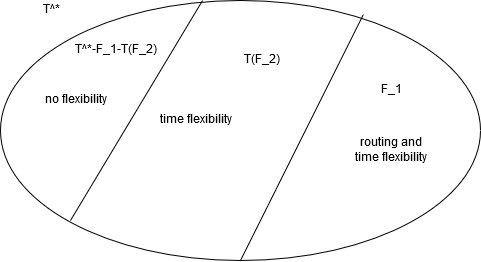
\includegraphics[width=0.7\textwidth]{flexibility.png}
	\caption{Degrees of flexibility for the Re-Scheduling-Problem.}
	\label{fig:ReSchedulingFlexi}
\end{figure}



A Solution $(\bar{P},\bar{A})$ of the Re-Scheduling Problem is a solution to the Scheduling Problem $(N^*,T^*,C^*)$, further satisfying
\begin{equation}
    \bar{P}(t) = P(t) \textrm{ for } t \not \in F_1,\label{eq:freedom_alternative_paths}
\end{equation}
\begin{equation}
    \bar{A}(t,v) = A(t,v) \textrm{ for } t \not \in F_1, t \not \in T(F_2), \label{eq:freedom_times_only}
\end{equation}
\begin{equation}
    \bar{A}(t,v^\prime) \geq S(t,v) \textrm { for all } S(t,v) \textrm{ and some } v^\prime \in W(_,v) \label{eq:respect_commercial_schedule}
\end{equation}
as well as equations (\ref{eq:path_consistency}),
(\ref{eq:start_and_target_node}), 
(\ref{eq:minimum_running_time_requirement}), 
(\ref{eq:mutual_resource_allocation_requirement}), 
(\ref{eq:connection_requirement}) above and minimizing
\begin{equation}
    \sum_{(t,v) \in \dom(S)} \bar{A}(t,v) -S(t,v).
\end{equation}
The Re-Scheduling Oracle defines the degrees of freedom on two levels, allowing path alternatives for trains $t\in F_1$ and allowing for modified departure times for the departures in $F_2$, but we require trains to respect the Commercial Schedule, i.e. we do not allow for trains or stops to be dropped.

\section{Results Hypothesis 1}

\subsection{Implementation Details}
k shortest paths, constraints in the model above, best-case Oracle

Our setting for Re-Scheduling for step XX in \cite{DBLP:journals/corr/abs-1807-11876}:
\begin{itemize}
    \item $N^*=N$
    \item $T$ = shortest path or all routes
    \item $C^*=C$
    \item $F_1$, $F_2$?
\end{itemize}{}

\section{Results Hypothesis 2}
\subsection{DL approaches}

\subsubsection{Graph-based Neighborhood Search (GNN)}
Approach Christian B. + Mayra

\subsubsection{Probabilistic Schedule (GNN)}
Erik

\subsubsection{Reinforcement Learning}
Erik with Jakab/Levent?

\subsection{Heuristics Oracle}

\subsubsection{Deadlock Avoidance}
Extending Adrian's Deadlock-Avoidance Algorithm? Christian E. and Adrian?



\subsubsection{Job Insertion}
Blocking Job-Shop-Scheduling Fribourg (Reinhard Bürgy)? Christian E. with Reinhard?

\subsection{Exploiting the Oracle in OR}
Christian E.

\section{Conclusion}
What have we achieved?

\section{Future Work}
Describe the Research Plan and the Challenge for other Researcher.


\section*{To Discuss}
\begin{itemize}
    \item definition of operational schedule should be independent of the scheduling problem based on time windows, definition is not very readable
    \item - not use $t$ for train but for time? Confusing for physicists....
    \item use real numbers for event times
    \item which cost function (classes) do we want to consider?
    \item use different mathematical problem formulation (alternative/disjunctive graph job shop scheduling,....?)
    \item Further Research: not only consider isolated events?
    \item Further Research: drop trains, drop halts, ...
    \item Further Research distributions or time windows as prognosis not only fixed event time
\end{itemize}


\bibliographystyle{unsrt}
\bibliography{biblio}

\end{document}
